% Sostituisco i placeholder registrati con la specifica variabile per il documento corrente. Questa parte iniziale contiene intestazioni e templates.

% Modificare ad ogni modifica e documento
\newcommand{\documento}{Manuale Utente}
\newcommand{\nomedocumentofisico}{ManualeUtente 2\_0\_0.pdf}
\newcommand{\redazione}{\MC \\ &  \DAN \\ &  \NS \\ & \DS \\ & \AS}
\newcommand{\verifica}{\AS}
\newcommand{\versione}{2.0.0}
\newcommand{\approvazione}{\DAN}
\newcommand{\uso}{Esterno}
\newcommand{\destinateTo}{\TV, \\ & \RC, \\ & \gruppo}
\newcommand{\datacreazione}{14 Aprile 2016}
\newcommand{\datamodifica}{15 giugno 2017}
\newcommand{\stato}{Approvato}

%Abilitazione indice delle tabelle e figure
\def\TABELLE{false}
\def\FIGURE{false}

%Inclusione di layout e variabili (Non modificare)
%Stile e dimensione del documento
\documentclass[a4paper,11pt]{article}

%Pacchetti da importare
\usepackage{ifthen}
\usepackage[italian]{babel}
\usepackage[utf8]{inputenc}
\usepackage[T1]{fontenc}
\usepackage{float}
\usepackage{chapterbib}
\usepackage{graphicx}
\usepackage[a4paper,top=2.5cm,bottom=2.5cm,left=2.5cm,right=2.5cm]{geometry}
\usepackage[colorlinks=true, urlcolor=black, citecolor=black, linkcolor=black]{hyperref}
\usepackage{booktabs}
\usepackage{fancyhdr}
\usepackage{totpages}
\usepackage{tabularx, array}
\usepackage{dcolumn}
\usepackage{epstopdf}
\usepackage{booktabs}
\usepackage{fancyhdr}
\usepackage{longtable}
\usepackage{calc}
\usepackage{datatool}
\usepackage[bottom]{footmisc}
\usepackage{listings}
\usepackage{textcomp}
\usepackage{titlesec}
\usepackage{rotating}
\usepackage{multirow}
\usepackage{placeins}
\usepackage{color}
\usepackage[table,usenames,dvipsnames]{xcolor}
\usepackage{hyperref}
\usepackage{makecell}
\usepackage{breakurl}
\usepackage{hyperref}
\usepackage{multirow}
\usepackage{xcolor,colortbl}
\usepackage{afterpage}
\usepackage{mathtools}
\usepackage{verbatim} 
\usepackage[toc,page]{appendix}

%glossary code%
\usepackage[nonumberlist,xindy]{glossaries}

\newglossarystyle{myaltlistgroup}{%
	\setglossarystyle{altlistgroup}%
	\renewcommand*{\glsgroupheading}[1]{%
		
		\newpage
		\item\makebox[\linewidth]{\Large\textbf{\glsgetgrouptitle{##1}}}%
		\vspace*{-\baselineskip}%
		\item\makebox[\linewidth]{\hspace*{3cm}\hrulefill\hspace*{3cm}}%
	}%
}



%Stile fancy per il documento (Header e footer)
\pagestyle{fancy}
%Rimuovo l'indentazione
\setlength{\parindent}{0pt}

%Imposto l'intestazione
\lhead{\Large{\progetto} \\ \footnotesize{\documento}}
%Linea sotto l'intestazione
\renewcommand{\headrulewidth}{0.4pt} 

%Footer
\lfoot{\textit{\gruppoLink}\\ \footnotesize{\email}}
%Footer con numero romano per le prime pagine
\rfoot{\thepage}
\cfoot{}
%Linea sopra il footer
\renewcommand{\footrulewidth}{0.4pt}   

%Imposta il livello degli elenchi 
\setcounter{secnumdepth}{7}
\setcounter{tocdepth}{7}

%Paragrafi impostati come una sezione
\titleformat{\paragraph}{\normalfont\normalsize\bfseries}{\theparagraph}{1em}{}
\titlespacing*{\paragraph}{0pt}{3.25ex plus 1ex minus .2ex}{1.5ex plus .2ex}

\titleformat{\subparagraph}{\normalfont\normalsize\bfseries}{\thesubparagraph}{1em}{}
\titlespacing*{\subparagraph}{0pt}{3.25ex plus 1ex minus .2ex}{1.5ex plus .2ex}

\makeatletter
\newcounter{subsubparagraph}[subparagraph]
\renewcommand\thesubsubparagraph{
  \thesubparagraph.\@arabic\c@subsubparagraph}
\newcommand\subsubparagraph{
  \@startsection{subsubparagraph}
    {6}
    {\parindent}
    {3.25ex \@plus 1ex \@minus .2ex}
    {0.75em}
    {\normalfont\normalsize\bfseries}}
\newcommand\l@subsubparagraph{\@dottedtocline{6}{10em}{5.5em}} 
\newcommand{\subsubparagraphmark}[1]{}
\makeatother

\makeatletter
\newcounter{subsubsubparagraph}[subsubparagraph]
\renewcommand\thesubsubsubparagraph{
  \thesubsubparagraph.\@arabic\c@subsubsubparagraph}
\newcommand\subsubsubparagraph{
  \@startsection{subsubsubparagraph}
    {7}
    {\parindent}
    {3.25ex \@plus 1ex \@minus .2ex}
    {0.75em}
    {\normalfont\normalsize\bfseries}}
\newcommand\l@subsubsubparagraph{\@dottedtocline{7}{10em}{6.5em}}
\newcommand{\subsubsubparagraphmark}[1]{}
\makeatother

\renewcommand\appendixtocname{Appendice}
\renewcommand\appendixpagename{Appendice}
%Variabili generali
\newcommand{\progetto}{API Market}
\newcommand{\gruppo}{NetBreak}
\newcommand{\gruppoLink}{\href{https://git.io/v1Rgz}{NetBreak}}
\newcommand{\email}{netbreakswe@gmail.com}

%Variabili riguardanti i documenti
\newcommand{\AdR}{Analisi dei Requisiti}
\newcommand{\NdP}{Norme di Progetto}
\newcommand{\PdP}{Piano di Progetto}
\newcommand{\SdF}{Studio di Fattibilità}
\newcommand{\PdQ}{Piano di Qualifica}
\newcommand{\VE}{Verbale}
\newcommand{\ST}{Specifica Tecnica}
\newcommand{\DDP}{Definizione di Prodotto}
\newcommand{\MU}{Manuale Utente}
\newcommand{\G}{Glossario}
\newcommand{\LdP}{Lettera di Presentazione}

%Variabili per i membri del gruppo
\newcommand{\AS}{Andrea Scalabrin}
\newcommand{\NS}{Nicolò Scapin}
\newcommand{\AN}{Alberto Nicolè}
\newcommand{\DS}{Davide Scarparo}
\newcommand{\DAN}{Dan Serbanoiu}
\newcommand{\MC}{Marco Casagrande}

%Ruoli di progetto
\newcommand{\RdP}{Responsabile di Progetto}
\newcommand{\Res}{Responsabile}
\newcommand{\Amm}{Amministratore}
\newcommand{\Ver}{Verificatore}
\newcommand{\Prog}{Progettista}
\newcommand{\Progr}{Programmatore}
\newcommand{\Ana}{Analista}
\newcommand{\RdPs}{Responsabili di Progetto}
\newcommand{\Ress}{Responsabile}
\newcommand{\Amms}{Amministratori}
\newcommand{\Vers}{Verificatori}
\newcommand{\Progs}{Progettisti}
\newcommand{\Progrs}{Programmatori }
\newcommand{\Anas}{Analisti}

%Professori e proponente
\newcommand{\TV}{Prof. Tullio Vardanega}
\newcommand{\RC}{Prof. Riccardo Cardin}
\newcommand{\IS}{ItalianaSoftware S.r.l.}
\newcommand{\proponente}{ItalianaSoftware S.r.l.}

\newcommand{\diaryEntry}[5]{#2 & \emph{#4} & #3 & #5 & #1\\ \hline}

%Comando per una nuova riga nella tabella del changelog
\newcommand{\specialcell}[2][c]{%
	\begin{tabular}[#1]{@{}c@{}}#2\end{tabular}}

\renewcommand*\sectionmark[1]{\markboth{#1}{}}
\renewcommand*\subsectionmark[1]{\markright{#1}}

%Variabili per la fase di lavoro
\newcommand{\AR}{Analisi dei Requisiti}
\newcommand{\ARD}{Analisi dei Requisiti Dettagliata}
\newcommand{\PA}{Progettazione Architetturale}
\newcommand{\PD}{Progettazione Architetturale Dettagliata}
\newcommand{\CO}{Codifica}
\newcommand{\VV}{Verifica e Validazione}

%Variabili per le varie revisioni
\newcommand{\RR}{Revisione dei Requisiti}
\newcommand{\RP}{Revisione di Progettazione}
\newcommand{\RPMin}{Revisione di Progettazione Minima}
\newcommand{\RPMax}{Revisione di Progettazione Massima}
\newcommand{\RQ}{Revisione di Qualifica}
\newcommand{\RA}{Revisione di Accettazione}

\newcommand{\myincludegraphics}[2][]{%
	\setbox0=\hbox{\phantom{X}}%
	\vtop{
		\hbox{\phantom{X}}
		\vskip-\ht0
		\hbox{\includegraphics[#1]{#2}}}}

\renewcommand\footnoterule{\rule{\linewidth}{1pt}}

\newcommand{\nogloxy}[1]{#1} % comando da usare per evitare di metttere il mark del glossario
\newcommand{\gloxy}[1]{\emph{#1}$_G$}

\colorlet{punct}{red!60!black}
\definecolor{background}{HTML}{EEEEEE}
\definecolor{delim}{RGB}{20,105,176}
\colorlet{numb}{magenta!60!black}
\lstdefinelanguage{json}{
	basicstyle=\small\ttfamily,
	numbers=left,
	numberstyle=\scriptsize,
	stepnumber=1,
	numbersep=8pt,
	showstringspaces=false,
	breaklines=true,
	frame=lines,
	backgroundcolor=\color{background},
	literate=
	*{0}{{{\color{numb}0}}}{1}
	{1}{{{\color{numb}1}}}{1}
	{2}{{{\color{numb}2}}}{1}
	{3}{{{\color{numb}3}}}{1}
	{4}{{{\color{numb}4}}}{1}
	{5}{{{\color{numb}5}}}{1}
	{6}{{{\color{numb}6}}}{1}
	{7}{{{\color{numb}7}}}{1}
	{8}{{{\color{numb}8}}}{1}
	{9}{{{\color{numb}9}}}{1}
	{:}{{{\color{punct}{:}}}}{1}
	{,}{{{\color{punct}{,}}}}{1}
	{\{}{{{\color{delim}{\{}}}}{1}
	{\}}{{{\color{delim}{\}}}}}{1}
	{[}{{{\color{delim}{[}}}}{1}
	{]}{{{\color{delim}{]}}}}{1},
}
\lstset{language=json}
\lstset{literate=%
	{Ö}{{\"O}}1
	{Ä}{{\"A}}1
	{Ü}{{\"U}}1
	{é}{{\"s}}1
	{è}{{\"e}}1
	{à}{{\"a}}1
	{ö}{{\"o}}1
}

\newcommand{\impl}{\textcolor{Green}{Implementato}}
\newcommand{\implno}{\textcolor{Red}{Non Implementato}}
\newcommand\Tstrut{\rule{0pt}{3.2ex}}         % = `top' strut
\newcommand\Bstrut{\rule[-1.9ex]{0pt}{0pt}}   % = `bottom' strut
\definecolor{Gray}{gray}{0.85}
\usepackage[inline]{enumitem}

%Inclusione del changelog per il documento corrente

\newcommand{\modifiche}
{
	Approvazione del documento & \specialcell[t]{\AS\\\Res} & \specialcell[t]{2017-01-04\\1.0.0}
	\\
	\midrule
	Verifica del documento & \specialcell[t]{\DS \\ \AN \\\Vers} & \specialcell[t]{2016-12-13\\0.3.0}
	\\
	\midrule
	Modifiche minori sulla base della verifica & \specialcell[t]{\AS\\\Res} & \specialcell[t]{2016-12-10\\0.2.2}
	\\
	\midrule
	Modifiche alla sezione Capitolato C3 & \specialcell[t]{\NS\\\Ana} & \specialcell[t]{2016-12-08\\0.2.1}
	\\
	\midrule
	Verifica del documento & \specialcell[t]{\AN\\\Ver} & \specialcell[t]{2016-12-07\\0.2.0}
	\\
	\midrule
	Modifiche dei paragrafi sulla base della verifica & \specialcell[t]{\AS\\\Res} & \specialcell[t]{2016-12-06\\0.1.1}
	\\
	\midrule
	Verifica del documento & \specialcell[t]{\DS\\\Ver} & \specialcell[t]{2016-12-06\\0.1.0}
	\\
	\midrule
	Accorpati i documenti e modifiche minori & \specialcell[t]{\AS\\\Res} & \specialcell[t]{2016-12-05\\0.0.9}
	\\
	\midrule
	Stesura del capitolato C2 & \specialcell[t]{\MC\\\Ana} & \specialcell[t]{2016-12-03\\0.0.8}
	\\
	\midrule
	Stesura del capitolato C5 & \specialcell[t]{\AN\\\Ana} & \specialcell[t]{2016-12-03\\0.0.7}
	\\
	\midrule
	Stesura del capitolato C4 & \specialcell[t]{\DS\\\Ana} & \specialcell[t]{2016-12-03\\0.0.6}
	\\
	\midrule
	Stesura del capitolato C3 & \specialcell[t]{\NS\\\Ana} & \specialcell[t]{2016-12-03\\0.0.5}
	\\
	\midrule
	Stesura del capitolato C6 & \specialcell[t]{\DAN\\\Ana} & \specialcell[t]{2016-12-03\\0.0.4}
	\\
	\midrule	
	Stesura del capitolato C1 & \specialcell[t]{\AS\\\Ana} & \specialcell[t]{2016-12-02\\0.0.3}
	\\
	\midrule
	Stesura dell'introduzione & \specialcell[t]{\AS\\\Ana} & \specialcell[t]{2016-12-02\\0.0.2}
	\\
	\midrule
	Creato template documento & \specialcell[t]{\AS\\\Ana} & \specialcell[t]{2016-12-02\\0.0.1}
	\\	
}


%Imposto la profondità degli indici
\setcounter{secnumdepth}{7}
\setcounter{tocdepth}{7}

\begin{document}

%Inclusione del template per la homepage (Non modificare)
%Importante: Non modificare questo template
%Modificare il documento principale per cambiare le parti

\begin{center}


%Spaziatura verticale

\vspace{4em}

%Intestazione con nome del gruppo
\begin{center} 
	\begin{Huge}
		\textbf{\fontsize{15mm}{20mm}\selectfont \gruppoLink} 
	\end{Huge}
\end{center}

\begin{center}
	\begin{Large}
		\vspace{0.3em}
		\textbf{Progetto \progetto}
	\end{Large}
\end{center}

%Inclusione del logo

\includegraphics[keepaspectratio = true,width=6cm]{../../Template/img/LogoNetbreak.png}

%Prima pagina senza intestazione né piè di pagina	
\thispagestyle{empty}

%Le informazioni del documento sono ancorate a fine pagina
\vfill

%Nome del documento
\begin{Huge} \textbf{\documento} \end{Huge}

%Tabella centrale
\begin{center}
\large\textbf{Informazioni sul documento} \\ \vspace{2em}
\small
\begin{tabular}{r l}
	\textbf{Nome del documento} & \nomedocumentofisico \\
	\textbf{Data di creazione} & \datacreazione\\
	\textbf{Ultima modifica} & \datamodifica\\
	\textbf{Versione} & \versione\\
	\textbf{Stato} & \stato \\
	\textbf{Redatto da}	& \redazione\\
	\textbf{Verificato da}	& \verifica\\
	\textbf{Approvato da}	& \approvazione\\
	\textbf{Uso}  & \uso\\
	\textbf{Distribuzione} & \gruppo \\
	\textbf{Destinato a}  &  \destinateTo \\
	\textbf{Email di riferimento}  &  \email \\
\end{tabular}
\end{center}

\vspace{2em}

\normalsize
%Inclusione abstract
\textbf{Abstract\\} 
Questo documento contiene il \PdP\ relativo al prodotto \progetto\ determinato dal gruppo \gruppo.
\end{center}
\clearpage


%Registro delle modifiche e indice (Non modificare)
\pagenumbering{Roman}
\newpage
% Non modificare - Pagina di Layout per il changelog
\begin{center}
	\Large{\textbf{Changelog}}
	\\\vspace{0.5cm}
	\normalsize
	\begin{tabularx}{\textwidth}{cXcc}
		\textbf{Versione} & \textbf{Descrizione} & \textbf{Autore e Ruolo} & \textbf{Data}
		\\\toprule
		\modifiche
		\bottomrule
	\end{tabularx}
\end{center}

\newpage
%Inserisce il link all'indice
%\addcontentsline{toc}{section}{Indice}
\newpage
\tableofcontents
\clearpage 

%Se è stata impostata a true la variabile per la lista delle tabelle, la mostra
\ifthenelse{\equal{\TABELLE}{true}} 
{\listoftables \newpage}{}

%Se è stata impostata a true la variabile per la lista delle figure, la mostra
\ifthenelse{\equal{\FIGURE}{true}}
{\listoffigures \newpage}{}

%Da qui comincia la numerazione normale
\pagenumbering{arabic}

%Imposta il formato di visualizzazione
\rfoot{\thepage~di~\pageref{TotPages}}

%Inclusione delle varie sezioni di contenuto
%Introduzione e contenuti di ogni tipo

\newpage
\section{Introduzione}

\subsection{Scopo del documento}
Lo scopo del documento è quello di presentare una breve analisi di tutti i capitolati proposti, con le motivazioni che hanno portato il gruppo a scegliere il capitolato C1. Tutti i capitolati son stati analizzati con la medesima metodologia,  evidenziando le tecnologie necessarie, il dominio applicativo e le criticità, e dando un giudizio finale con le opinioni raccolte all'interno del gruppo.

\subsection{Scopo del prodotto}
Lo scopo del prodotto è la realizzazione di un \textit{API Market\ped{G}} per l'acquisto e la vendita di \textit{microservizi\ped{G}}. Il sistema offrirà la possibilità di registrare nuove \textit{API\ped{G}} per la vendita, permetterà la consultazione e la ricerca di API ai potenziali acquirenti, gestendo i permessi di accesso ed utilizzo tramite creazione e controllo di relative \textit{API key\ped{G}}. Il sistema, oltre alla web app stessa, sarà corredato di un \textit{API Gateway\ped{G}} per la gestione delle richieste e il controllo delle chiavi, e fornirà funzionalità avanzate di statistiche per il gestore della piattaforma e per i fornitori dei microservizi.

\subsection{Riferimenti normativi}
\begin{itemize}
	\item \textsc{NormeDiProgetto 2\_0\_0.pdf}
\end{itemize}

\subsection{Riferimenti informativi}
\begin{itemize}
	\item \textbf{Capitolato d'appalto C1:} APIM: An API Market Platform \\ \url{http://www.math.unipd.it/~tullio/IS-1/2016/Progetto/C1.pdf}
	\item \textbf{Capitolato d'appalto C2:} AtAVi: Accoglienza tramite Assistente Virtuale \\ \url{http://www.math.unipd.it/~tullio/IS-1/2016/Progetto/C2.pdf}
	\item \textbf{Capitolato d'appalto C3:} DeGeOP: A Designer and Geo-localizer Web App for Organizational Plants \\
	\url{http://www.math.unipd.it/~tullio/IS-1/2016/Progetto/C3.pdf}
	\item \textbf{Capitolato d'appalto C4:} eBread: applicazione di lettura per dislessici \\
	\url{http://www.math.unipd.it/~tullio/IS-1/2016/Progetto/C4.pdf}
	\item \textbf{Capitolato d'appalto C5:} Monolith: an interactive bubble provider \\
	\url{http://www.math.unipd.it/~tullio/IS-1/2016/Progetto/C5.pdf}
	\item \textbf{Capitolato d'appalto C6:} SWEDesigner: editor di diagrammi UML con generazione di codice \\
	\url{http://www.math.unipd.it/~tullio/IS-1/2016/Progetto/C6.pdf}
\end{itemize}

\subsection{Glossario}
Per semplificare la consultazione e disambiguare alcune terminologie tecniche, le voci indicate con la lettera \textit{G} a pedice sono descritte approfonditamente nel documento \textsc{Glossario 2\_0\_0.pdf} e specificate solo alla prima occorrenza all'interno del suddetto documento.
\newpage
\section{Modalità di utilizzo e requisiti}

\subsection{Categorie di utenza}
Sono presenti due categorie di utilizzo per l'utente. Esse permettono di accedere in modo differente alle varie aree del sito. Riassumiamo nell'elenco sottostante le categorie presentate:

\begin{itemize}
	\item \textbf{Utente non autenticato}: rappresenta l'utente che visita il sito per la prima volta oppure quando non ha effettuato il login nella piattaforma. All'utente non autenticato è permessa la visualizzazione dei prodotti inseriti nella piattaforma, così come la ricerca. Essi però non hanno accesso alle aree e funzionalità riservate;
	\item \textbf{Utente autenticato}: un utente appartenente a questa categoria possiede le funzionalità di ricerca come per l'utenza non autenticata. Inoltre, ha a disposizione il proprio profilo utente ed è abilitato all'acquisto dei servizi offerti nel sito, con l'accesso alle relative funzionalità statistiche;
	\item \textbf{Utente autenticato generico}: questa categoria di utente è una sottoclasse dell'utente autenticato, ma risulta abilitato all'inserimento e gestione dei propri servizi per la vendita ad altri utenti della piattaforma. 
\end{itemize}

Gli utenti registrati devono appartenere ad una categoria di utente. Queste categorie sono cliente, sviluppatore, amministratore.

Per semplicità di lettura il documento è stato suddiviso in tre sezioni, ognuna delle quali prende in esame le possibili azioni che un utente può svolgere nella piattaforma. Le categorie di utenti sono:
\begin{itemize}
	\item \textbf{Cliente}: rappresenta un utente registrato, che può acquistare ed utilizzare API;
	\item \textbf{Sviluppatore}: rappresenta un utente registrato che oltre a poter svolgere le stesse operazioni di un cliente, può caricare le proprie API su \textit{API Market} e trasferire i profitti su un conto Paypal;
	\item \textbf{Amministratore}: rappresenta un utente con priviliegi di moderazione che incidono sia su sviluppatori o clienti sia API.
\end{itemize}

\subsection{Requisiti di sistema}
APIM, essendo un applicazione web-based, richiede l'accesso ad internet per poter essere utilizzato. La compatibilità \textit{browser\ped{G}} è riassumibile nell'elenco sottostante, fermo restando che seppur non garantita potrebbe esserci compatibilità con versioni antecedenti a quelle indicate. L'utente per usufruire della piattaforma non deve installare alcun componente, ma deve attivare \textit{javascript\ped{G}} sul browser web scelto per usufruire dei contenuti della \textit{web app\ped{G}}.
L'hardware del dispositivo non è oggetto di vincolo all'utilizzo.

\subsubsection{Browser supportati}
Il software API Market supporta i browser a partire dalle versioni: \textit{Google Chrome\ped{G}} 56.0, Mozilla Firefox 51.0, Safari 10.0, Microsoft Edge 38.0, Android browser 5.1 e Safari per \textit{iOS\ped{G}} 10.





\newpage
\section{Utente Non Registrato o Loggato}

	\subsection{Homepage}
		La schermata principale dell'applicazione appare come mostrato nella figura sottostante ed è visibile a qualsiasi tipologia di utente.
		
		\label{Homepage}
		\begin{figure}[H]
			\centering
			\fbox{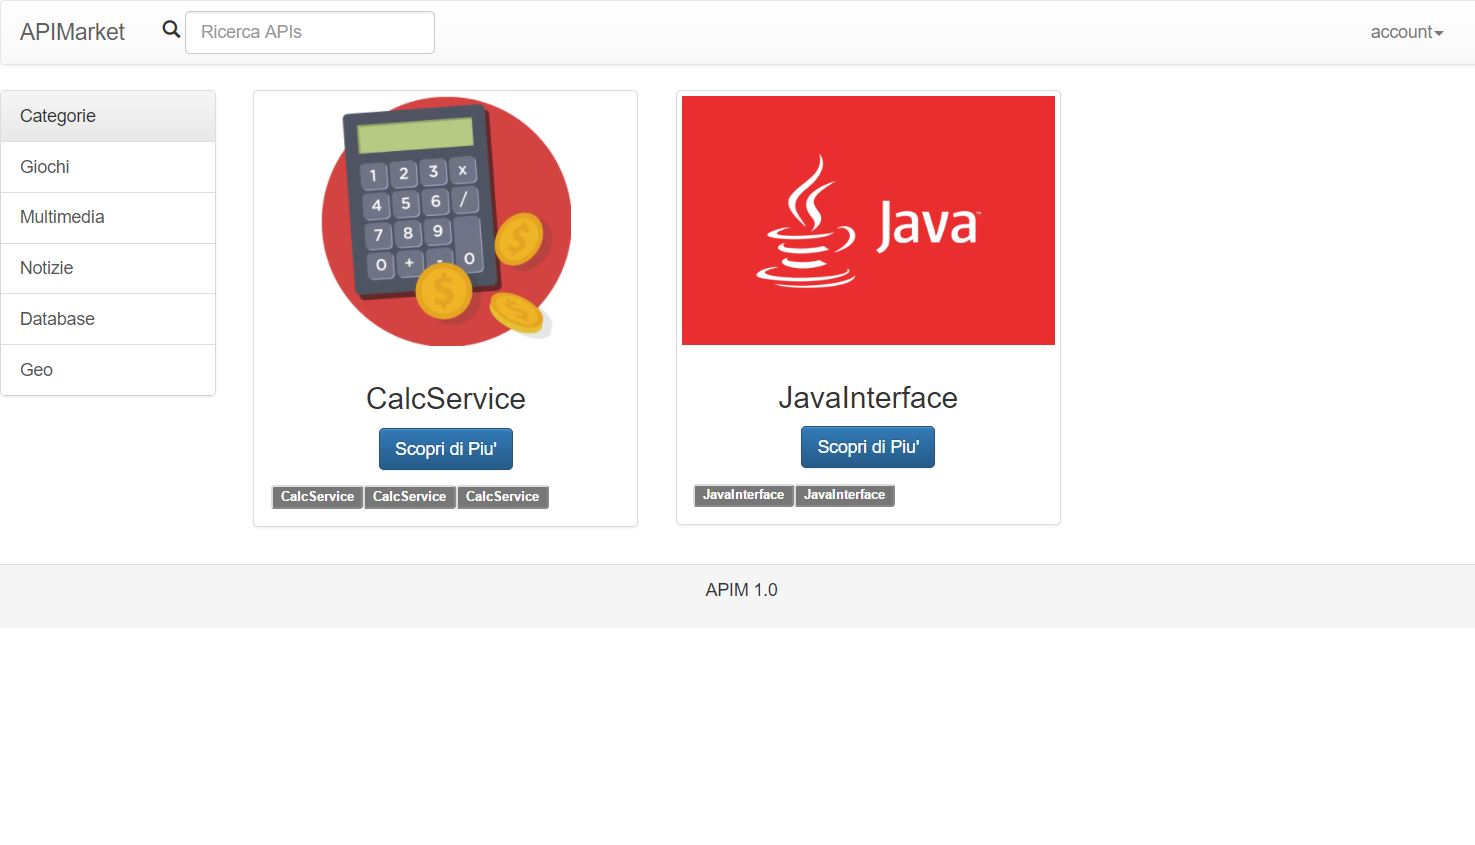
\includegraphics[scale=0.29]{img/APIM_home.JPG}}
			\caption{Homepage}
		\end{figure}
		
		Dalla schermata principale sono possibili le principali funzionalità dell'utente non autenticato. L'utente può registrarsi e autenticarsi tramite il menu in alto a destra, mentre a sinistra può sfogliare le varie categorie di API esposte nel market. Tramite la barra di ricerca, posta alla destra del logo del market, può effettuare una ricerca tramite keyword. Nella parte centrale dell'immagine sono disponibili le ultime otto API inserite all'interno dell'API Market.
		In fondo alla pagina è presente il footer, che contiene alcune informazioni sull'API Market.
		Come è possibile notare nella Figura 1, per la homepage, come per il resto della piattaforma è stato scelto un layout minimale e semplice per renderlo di facile utilizzo a diverse tipologie di utente.

	\subsection{Registrazione}
	Per poter usufruire delle funzionalità complete dell'API Market, quali acquisto e vendita di API, è necessario registrarsi. \MakeUppercase{è} possibile registrarsi alla piattaforma premendo il pulsante preposto nella barra superiore. La schermata che apparirà all'utente sarà la seguente:
	
	\label{Registrazione}
	\begin{figure}[H]
		\centering
		\fbox{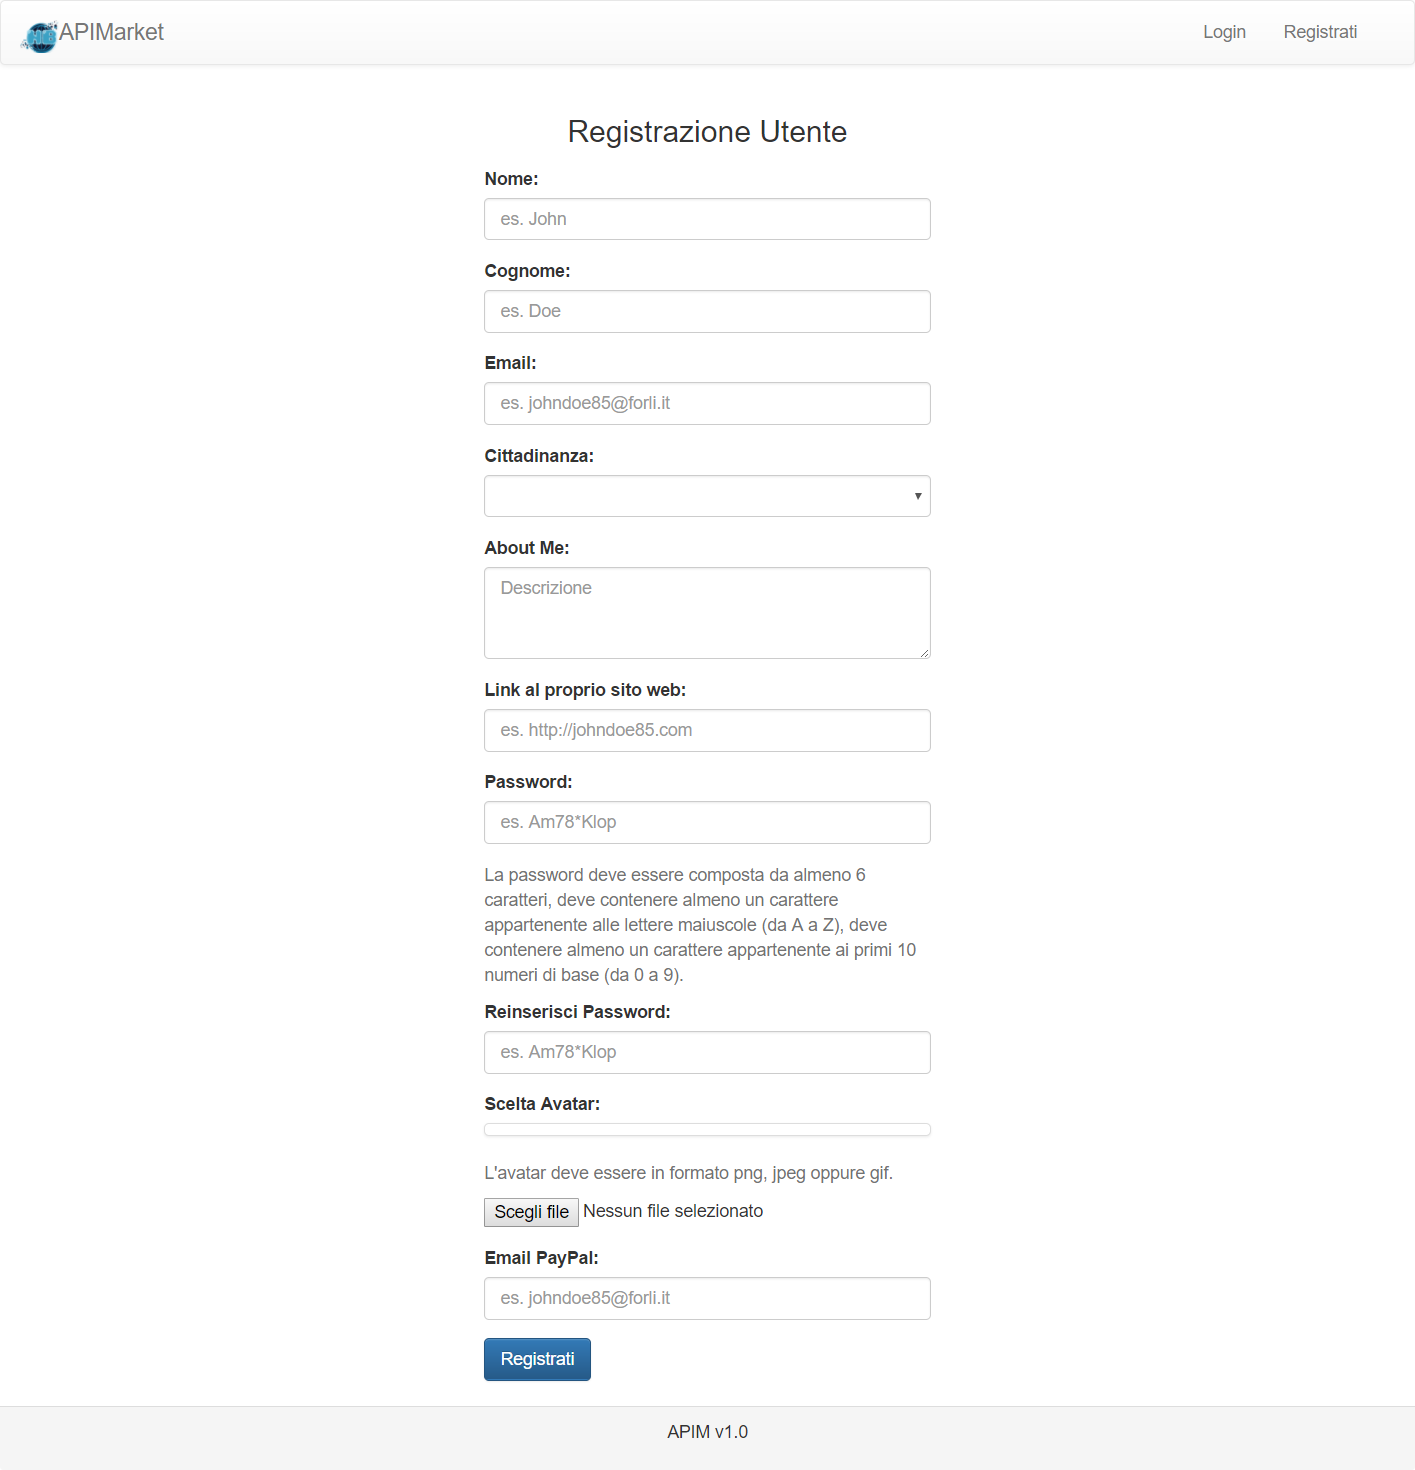
\includegraphics[scale=0.31]{img/APIM_registrazione.JPG}}
		\caption{Registrazione}
	\end{figure}
	
	Un utente per registrarsi dovrà compilare correttamente i seguenti campi, che sono obbligatori:
	\begin{itemize}
		\item Nome;
		\item Cognome;
		\item Username desiderato;
		\item Stato di residenza;
		\item Indirizzo e-mail;
		\item Password desiderata;
		\item Conferma password.
	\end{itemize}
	
	Qualora questi dati non fossero presenti o corretti, il sistema segnala un errore all'atto di registrazione e l'utente deve inserire dei parametri validi nei campi indicati. Sono presenti inoltre dei campi opzionali, destinati all'utente che vuole essere anche sviluppatore:
	
	\begin{itemize}
		\item Descrizione personale;
		\item Immagine personale;
		\item Email PayPal.
	\end{itemize}
	
	Questi campi, seppur non obbligatori, bloccano la registrazione qualora il loro inserimento non fosse effettuato in modo corretto. Si prega di prestare attenzione ai requisiti visualizzati nella schermata di registrazione.
	
	\subsection{Login}
	
	Tramite la barra superiore, vicino al pulsante di registrazione è possibile effettuare il login. La schermata di login può essere visualizzata a partire da ogni pagina non autenticata, selezionando l'apposita voce.
	Il login può essere effettuato da un utente precedentemente registrato e dalla schermata di login è possibile autenticarsi nella piattaforma per poter svolgere le funzionalità preposte agli utenti registrati. 
	
	\label{Login}
	\begin{figure}[H]
		\centering
		\fbox{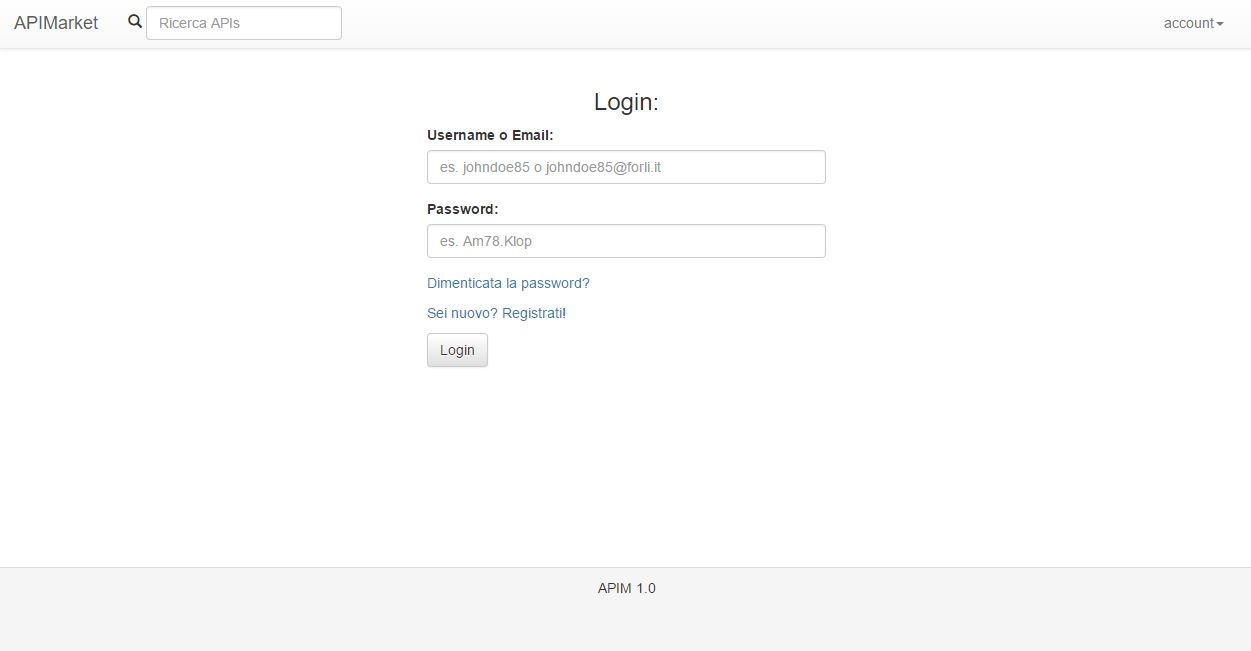
\includegraphics[scale=0.31]{img/APIM_login.JPG}}
		\caption{Login}
	\end{figure}
	
	\subsection{Conferma Login}
	Dopo aver inserito i dati di login e cliccato sul pulsante "Login", se i dati di accesso sono corretti, l'utente visualizza una pagina di conferma login, con la possibilità di recarsi sulla Homepage oppure nella gestione del proprio profilo.
	
	\label{Conferma Login}
	\begin{figure}[H]
		\centering
		\fbox{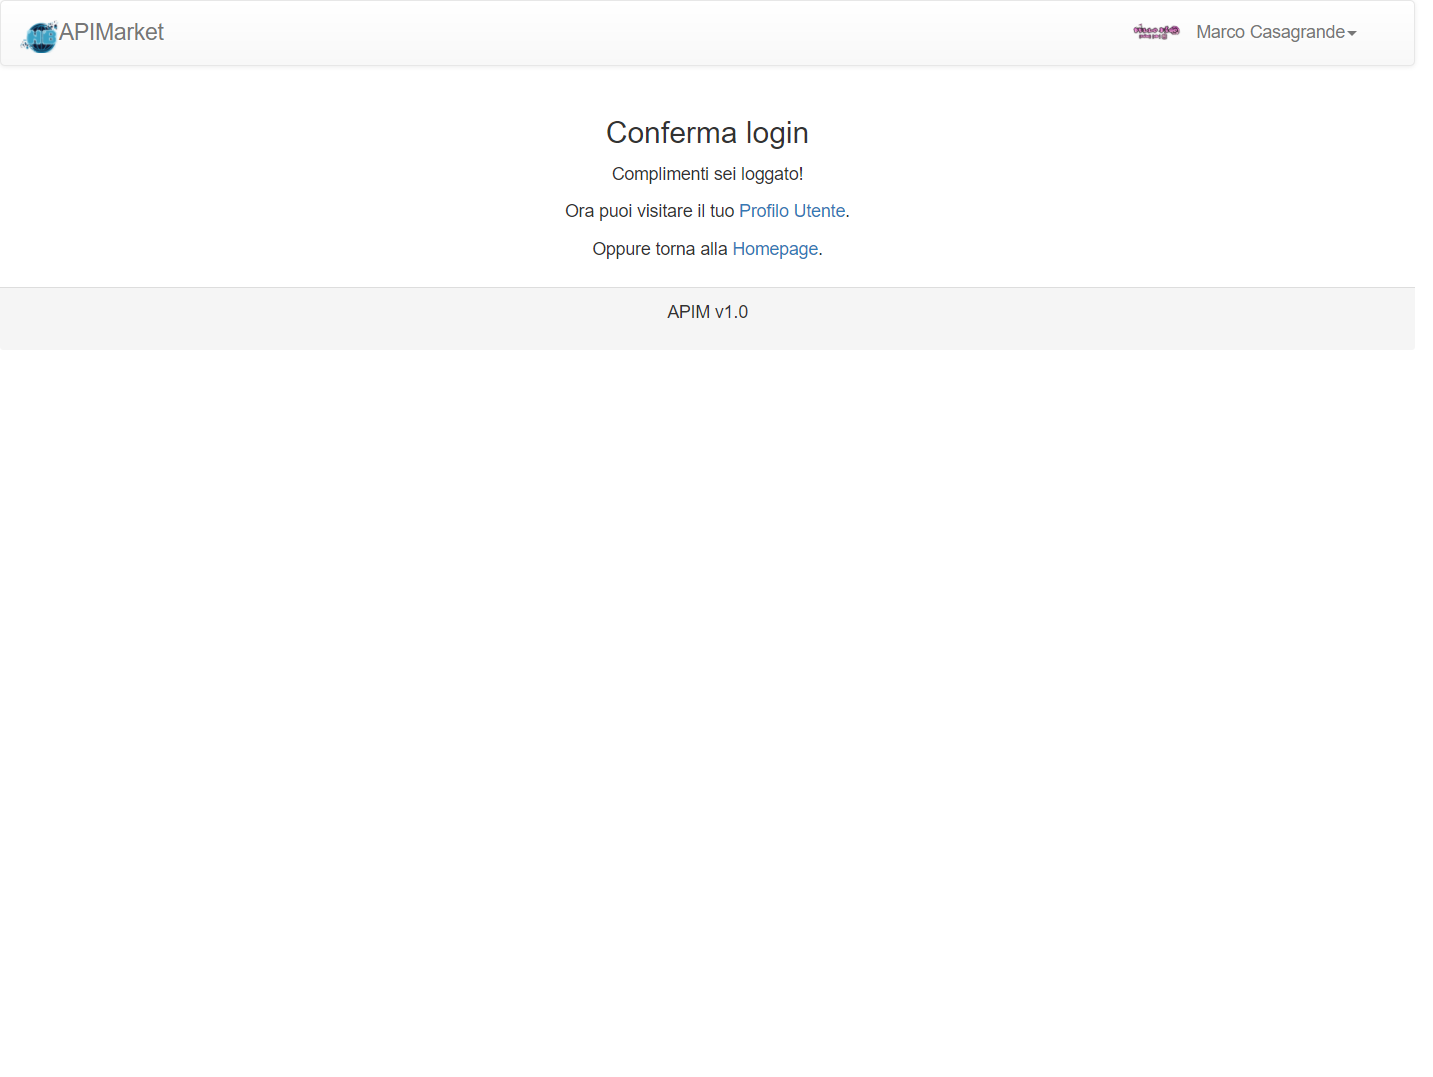
\includegraphics[scale=0.31]{img/APIM_confermaLogin.jpg}}
		\caption{Login}
	\end{figure}
	
	
	
	\subsection{Recupero Password}
	Qualora si fosse dimenticata la password, dalla schermata di login si può accedere alla pagina per il recupero della password. Inserendo l'indirizzo email si può ottenere un link per reimpostare i propri dati personali tramite una pagina dedicata. 
	
	\label{Recupero Password}
	\begin{figure}[H]
		\centering
		\fbox{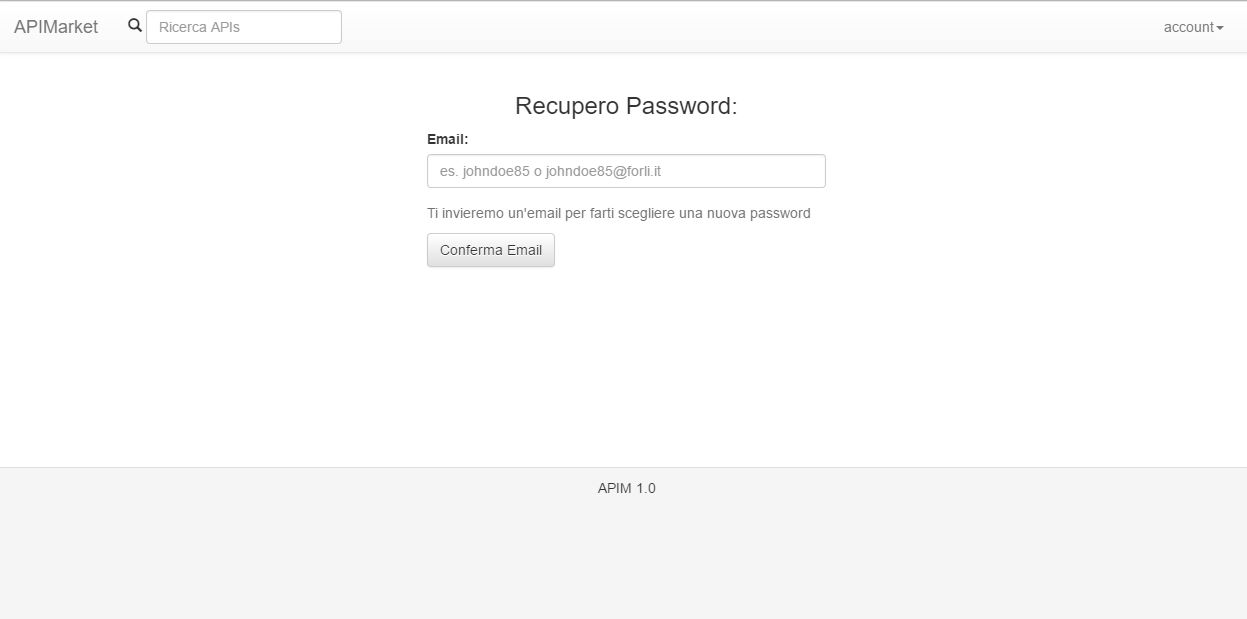
\includegraphics[scale=0.31]{img/APIM_recuperoPSW.JPG}}
		\caption{Recupero Password}
	\end{figure}

\subsection{Ricerca e visualizzazione API}

\subsubsection{Ricerca}
La funzionalità di ricerca è disponibile per qualsiasi categoria di utente. Essa permette, in base ad una parola chiave, di visualizzare le API relative contenute nella piattaforma. In seguito a ricerca, effettuata scrivendo sull'apposita barra la parola chiave desiderata, si può accedere ad un elenco dei risultati come mostrato. 

\label{Risultati ricerca}
\begin{figure}[H]
	\centering
	\fbox{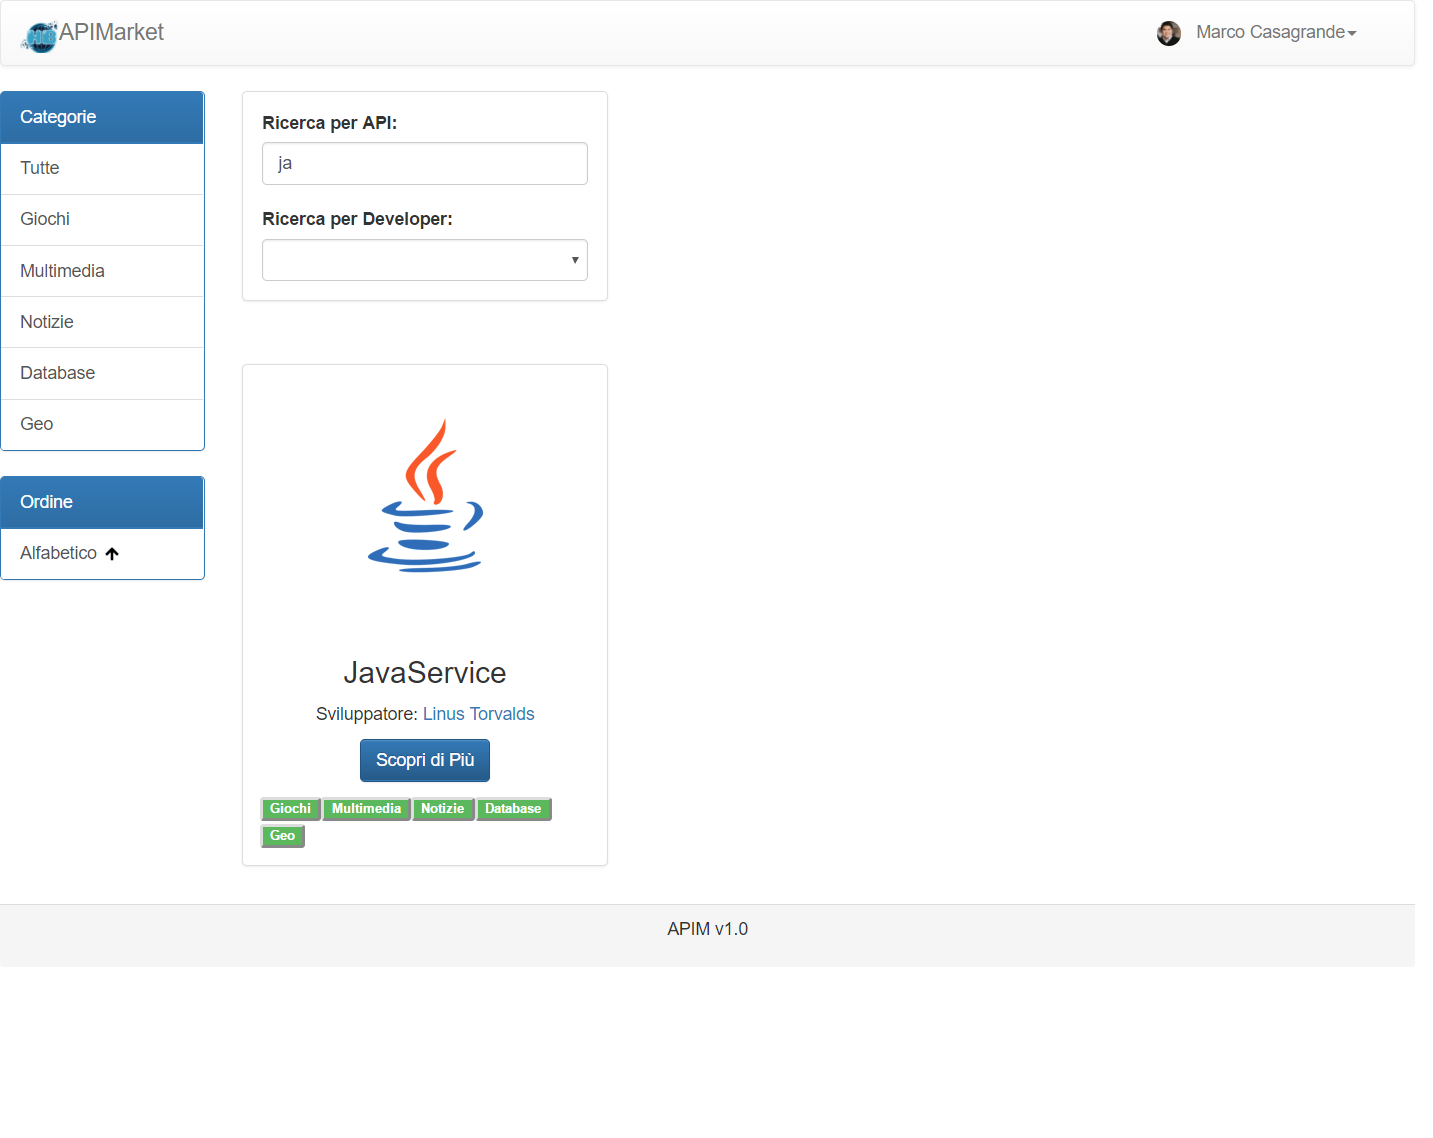
\includegraphics[scale=0.31]{img/APIM_ricerca.JPG}}
	\caption{Risultati ricerca}
\end{figure}


\subsubsection{Visualizzazione dettagli API}
Selezionando un API dall'elenco dei risultati, è possibile visualizzare i dati nel dettaglio, con relative specifiche. 


\label{Visualizzazione API}
\begin{figure}[H]
	\centering
	\fbox{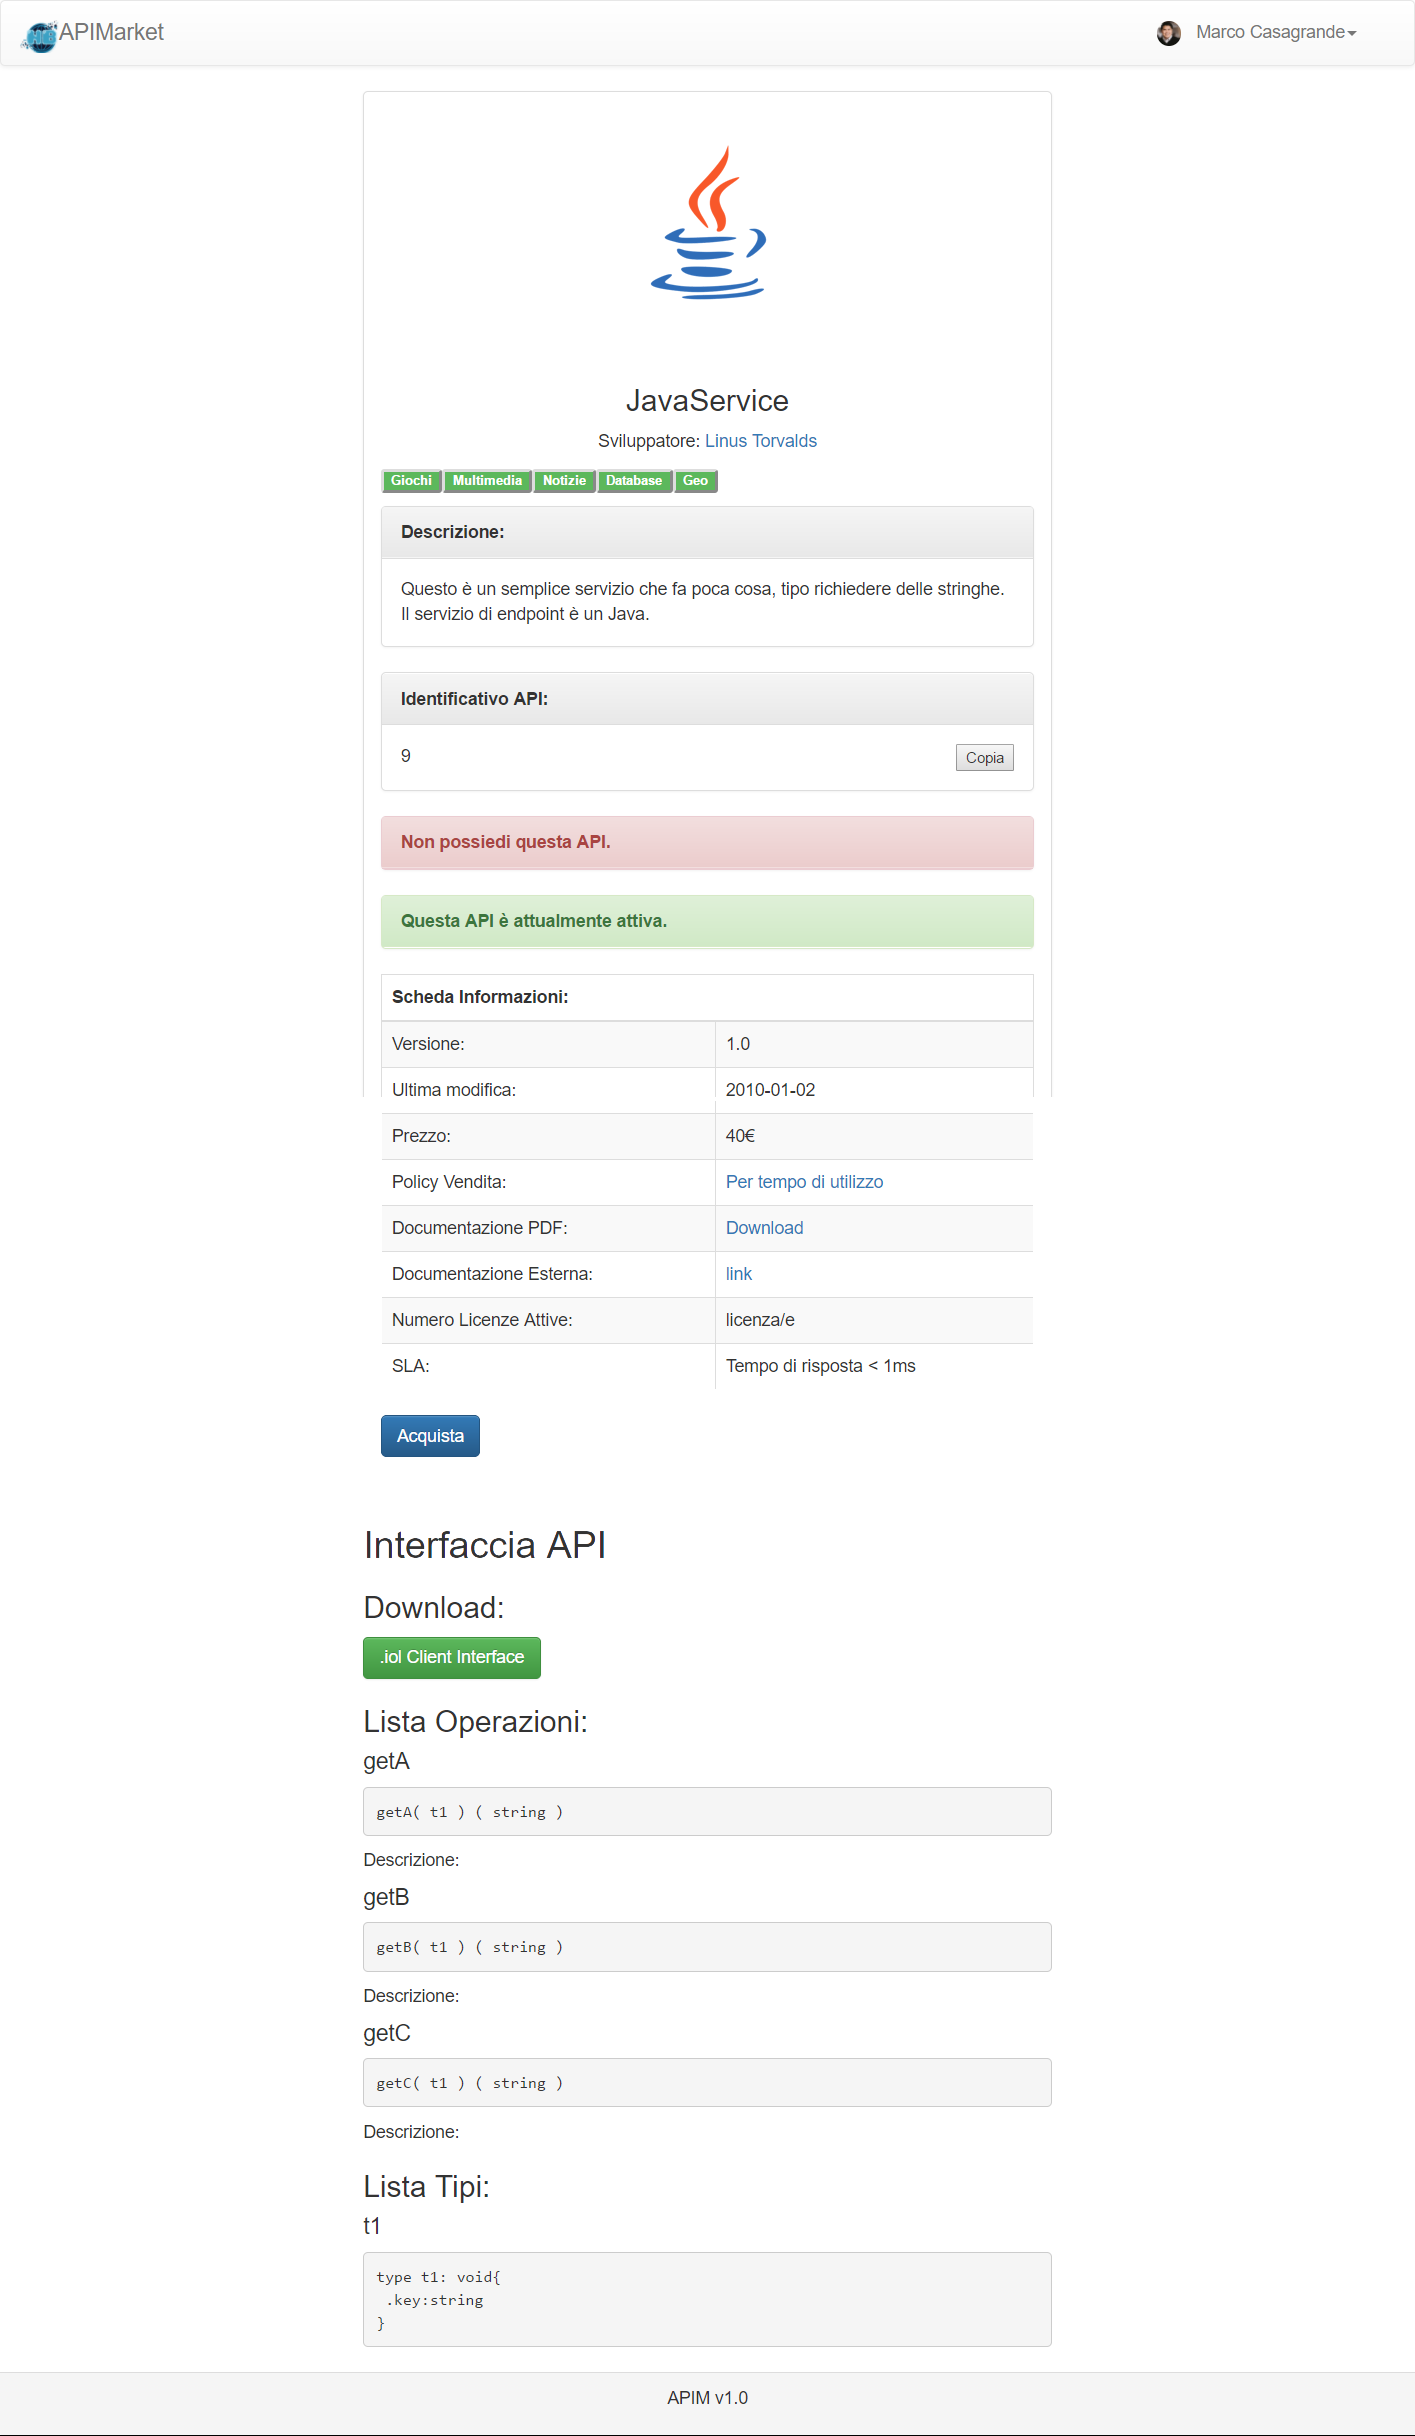
\includegraphics[scale=0.28]{img/APIM_dettagliApi.png}}
	\caption{Visualizzazione API}
\end{figure}

Ciascuna API presente nella piattaforma è caratterizzata da una policy di vendita, descritta all'interno di ciascun prodotto. E' possibile visualizzare i dettagli della policy clickando sull'apposito link nella schermata.

\label{Visualizza policy API}
\begin{figure}[H]
	\centering
	\fbox{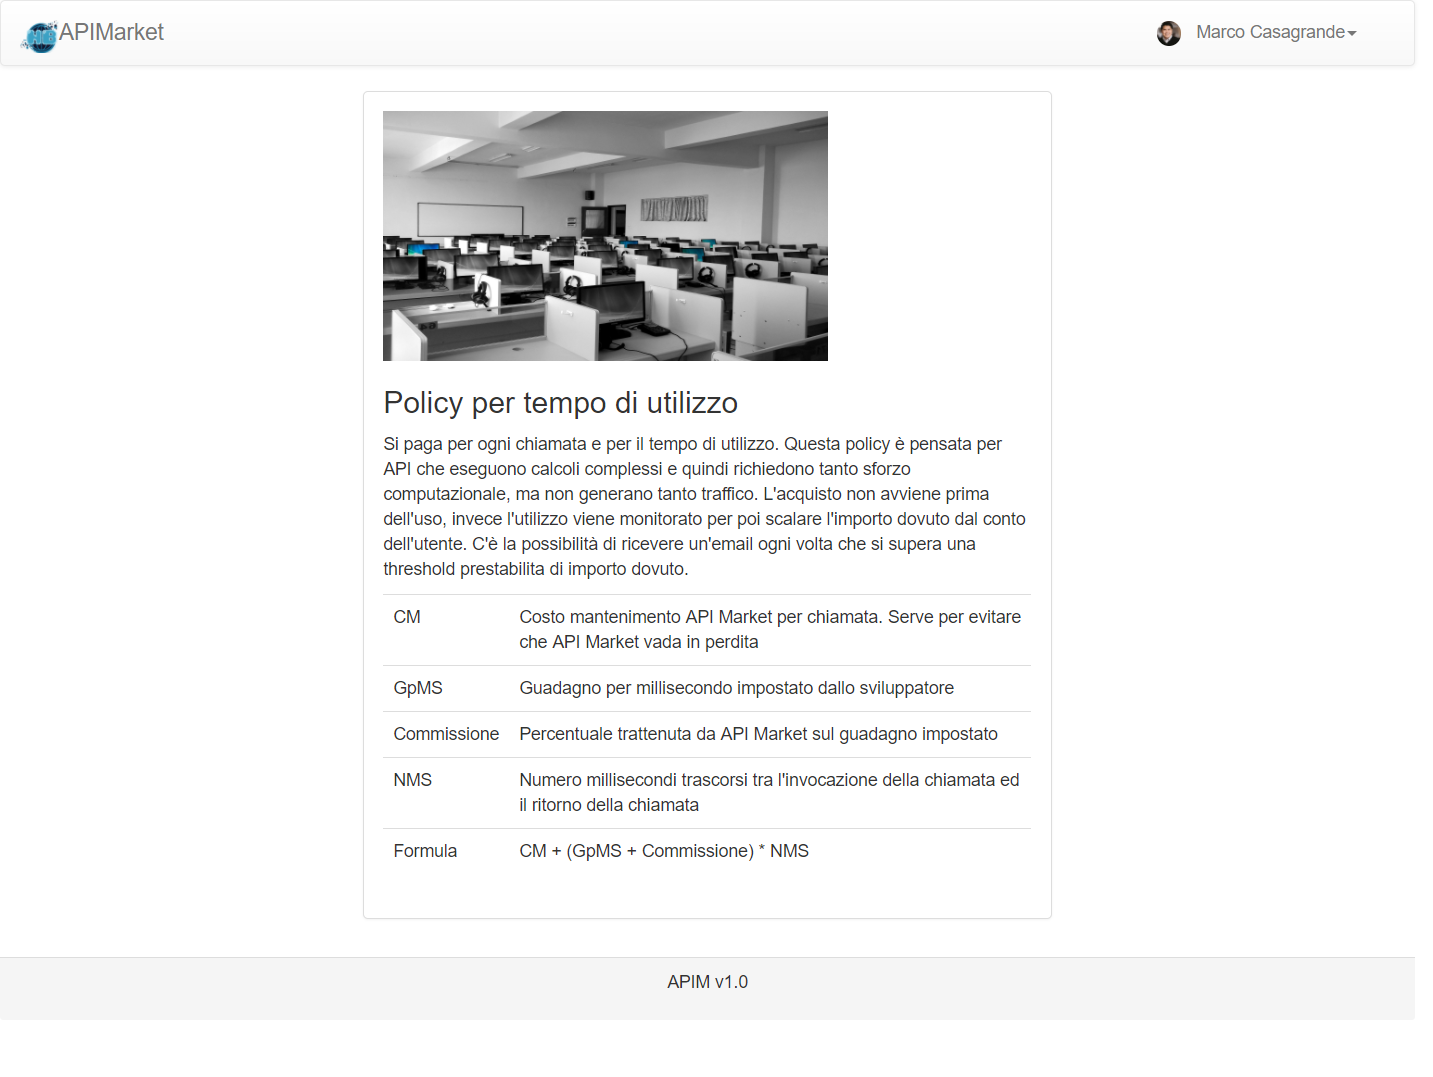
\includegraphics[scale=0.31]{img/APIM_policy.JPG}}
	\caption{Visualizza policy API}
\end{figure}

\subsubsection{Acquisto}
Qualora si decidesse di effettuare l'acquisto, nella schermata è presente un pulsante Acquista. Nella stessa schermata un utente loggato può inserire la quantità che intende acquistare, altrimenti chiederà di effettuare il login o la registrazione. Per maggiori relativi all'acquisto, si rimanda alla sezione 4.2 del presente manuale.





\newpage
\section{Cliente}

\subsection{Gestione profilo}

Una volta effettuato con successo il login, è possibile accedere al proprio profilo utente. La schermata principale relativa al profilo apparirà come nella figura sottostante.

\label{Profilo utente}
\begin{figure}[H]
	\centering
	\fbox{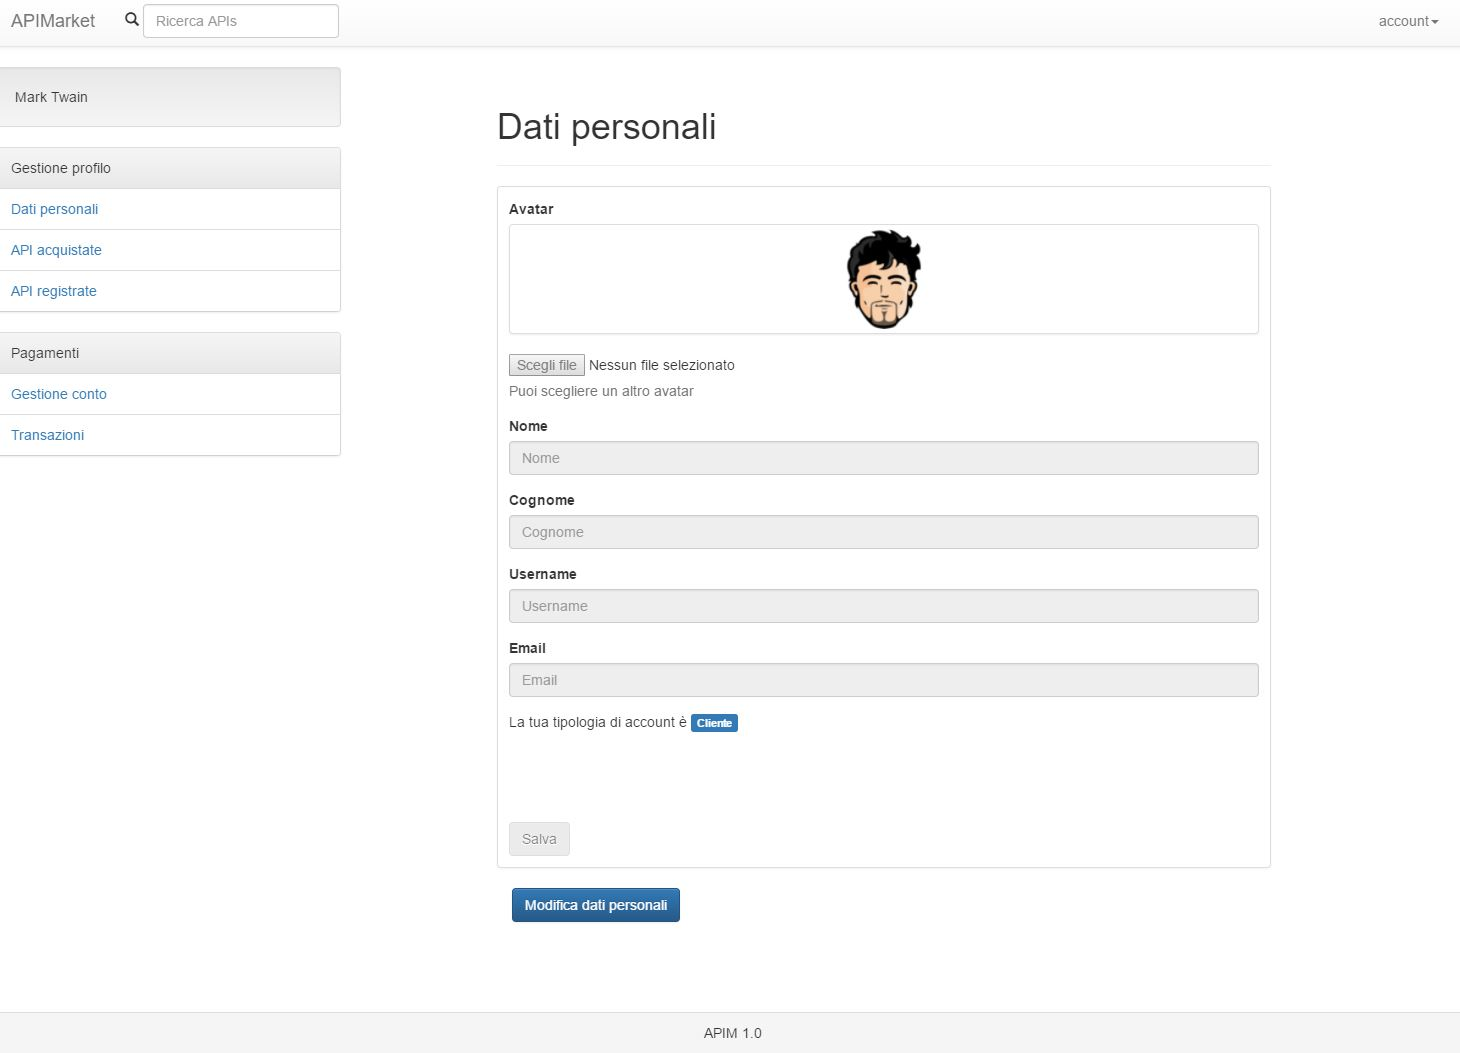
\includegraphics[scale=0.31]{img/APIM_account.JPG}}
	\caption{Profilo utente}
\end{figure}

Dalla schermata si potranno modificare i dati personali, inseriti al momento della registrazione, quali la propria anagrafica o dati relativi all'account quali l'immagine personale. E' visualizzato inoltre a quale gruppo di utenza si appartiene: l'utente registrato semplice infatti è un utente denominato "cliente", mentre l'utente abilitato al caricamento e alla vendita di servizi è denominato utente "Developer".

Tramite il menù laterale è possibile navigare nelle schermate del proprio profilo. Clickando sulla voce API acquistate si potrà consultare l'elenco delle api attualmente in possesso o acquistate in passato con i relativi dati. 

\label{API acquistate}
\begin{figure}[H]
	\centering
	\fbox{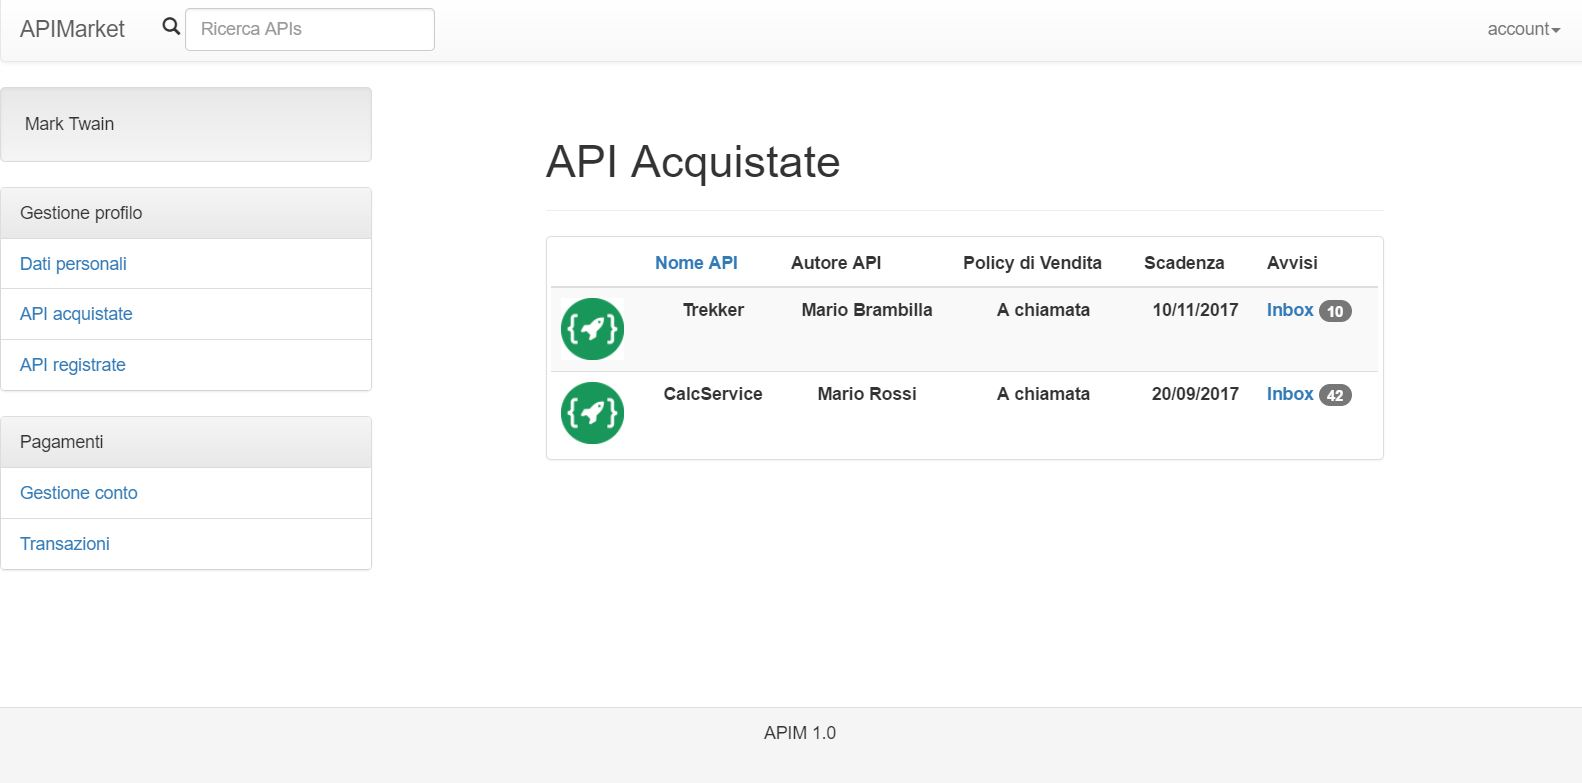
\includegraphics[scale=0.31]{img/APIM_apiAcquistate.JPG}}
	\caption{API acquistate}
\end{figure}
Nell'elenco delle API Acquistate è possibile rinnovare un'API prossima alla scadenza tramite l'apposito pulsante. L'utente effettuerà così una nuova transazione.


\subsection{Acquisto API}
Un cliente può acquistare una API direttamente dalla pagina di dettaglio API tramite il pulsante Acquista. 

All'interno della pagina relativa al completamento della transizione, l'utente potrà scegliere l'importo da acquistare a seconda della policy dell'API che intende acquistare.  

Una volta completata la transazione l'utente riceverà un API key con la quale potrà utilizzare il servizio acquistato. 

\label{Acquisto API}
\begin{figure}[H]
	\centering
	\fbox{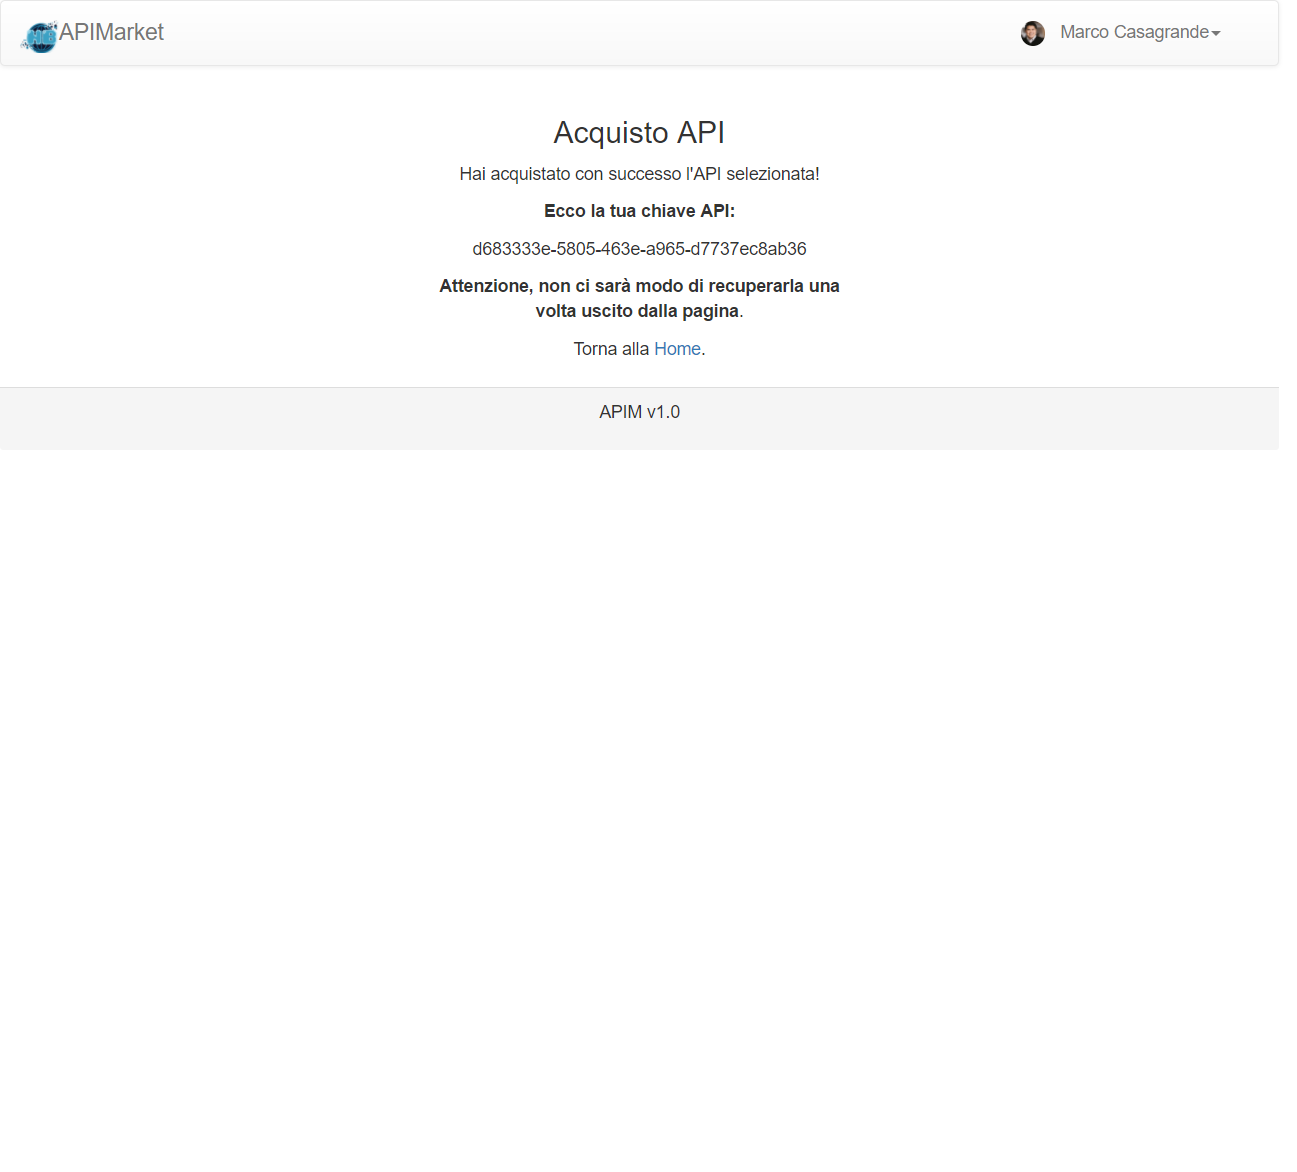
\includegraphics[scale=0.31]{img/APIM_confermaAcquisto.png}}
	\caption{Acquisto API}
\end{figure}

\subsection{Acquisto crediti}
Dalla gestione del profilo, un utente è in grado di acquistare crediti utilizzabili per pagare le API. Un utente può acquistare un numero di crediti a scelta tra i tagli presenti nell'apposita pagina. Nella pagina successiva l'utente completa la transazione e il saldo crediti del suo conto viene aggiornato con i nuovi crediti sommati ai precedenti.

\label{Acquisto Crediti}
\begin{figure}[H]
	\centering
	\fbox{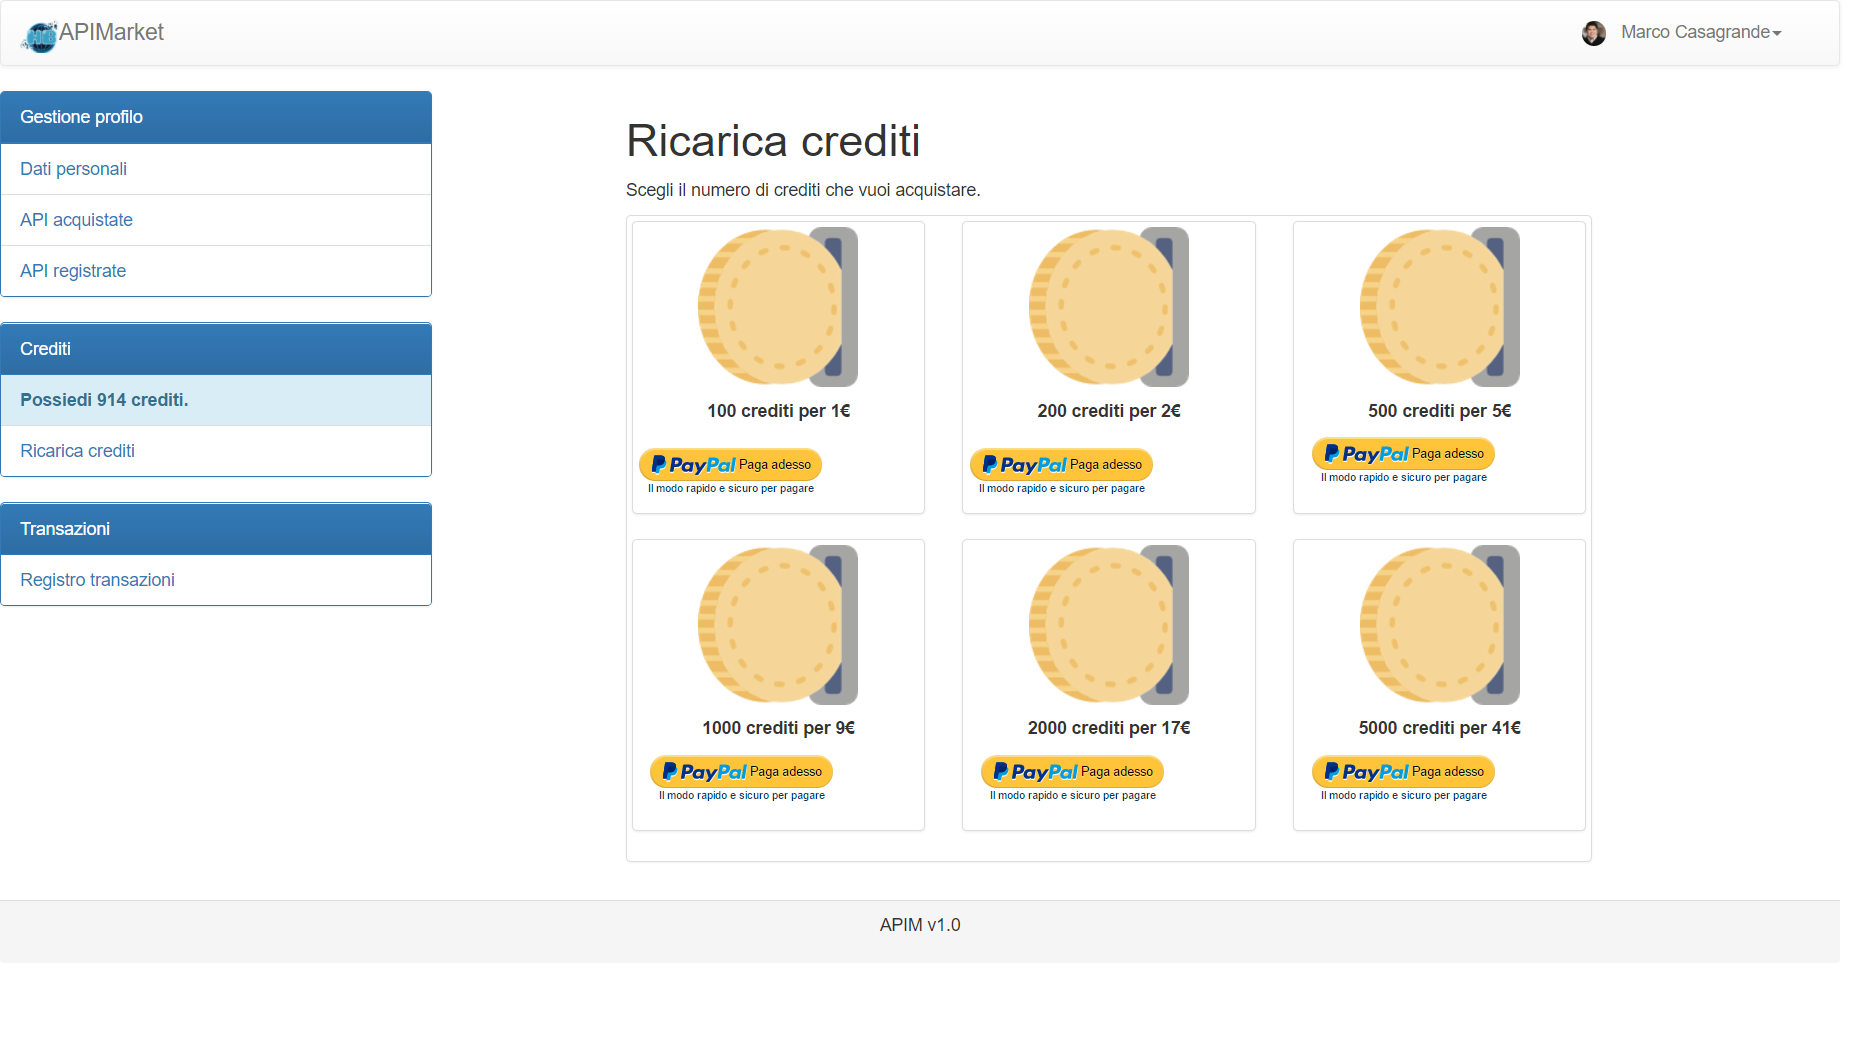
\includegraphics[scale=0.31]{img/APIM_acquistoCrediti.JPG}}
	\caption{Acquisto Crediti}
\end{figure}


\newpage
\section{Sviluppatore}
Lo sviluppatore è in grado di eseguire tutte le operazioni disponibili al cliente e in aggiunta può inserire API nel market e trasferire il guadagno proveniente dalla vendita nel suo saldo Paypal.
Uno sviluppatore deve inserire, se non fatto al momento della registrazione i seguenti dati obbligatori:
	
\begin{itemize}
	\item Descrizione personale;
	\item Immagine personale;
	\item Email PayPal.
\end{itemize}


\subsection{API registrate}
Lo sviluppatore all'interno della sua area personale può visualizzare le API registrate e le loro caratteristiche principali.

\label{API registrate}
\begin{figure}[H]
	\centering
	\fbox{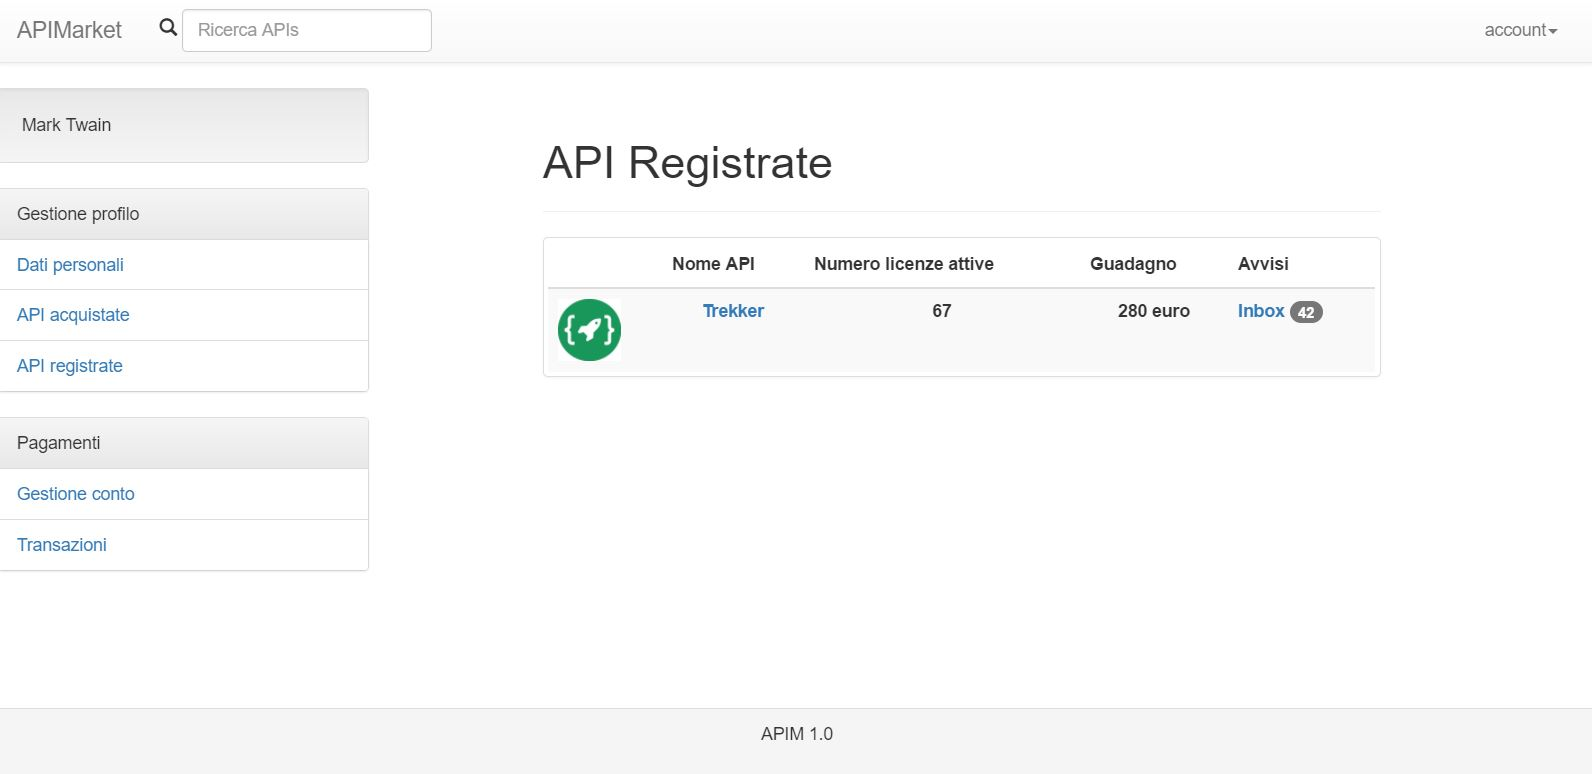
\includegraphics[scale=0.31]{img/APIM_apiRegistrate.JPG}}
	\caption{API registrate}
\end{figure}

\subsection{Registrazione API}

L'utente abilitato alla vendita (Sviluppatore) può  registrare le proprie API per la vendita nell'apposita pagina accessibile dal profilo utente. La schermata per la registrazione di nuove API appare come mostrato nell'immagine sottostante.

\label{Registrazione API}
\begin{figure}[H]
	\centering
	\fbox{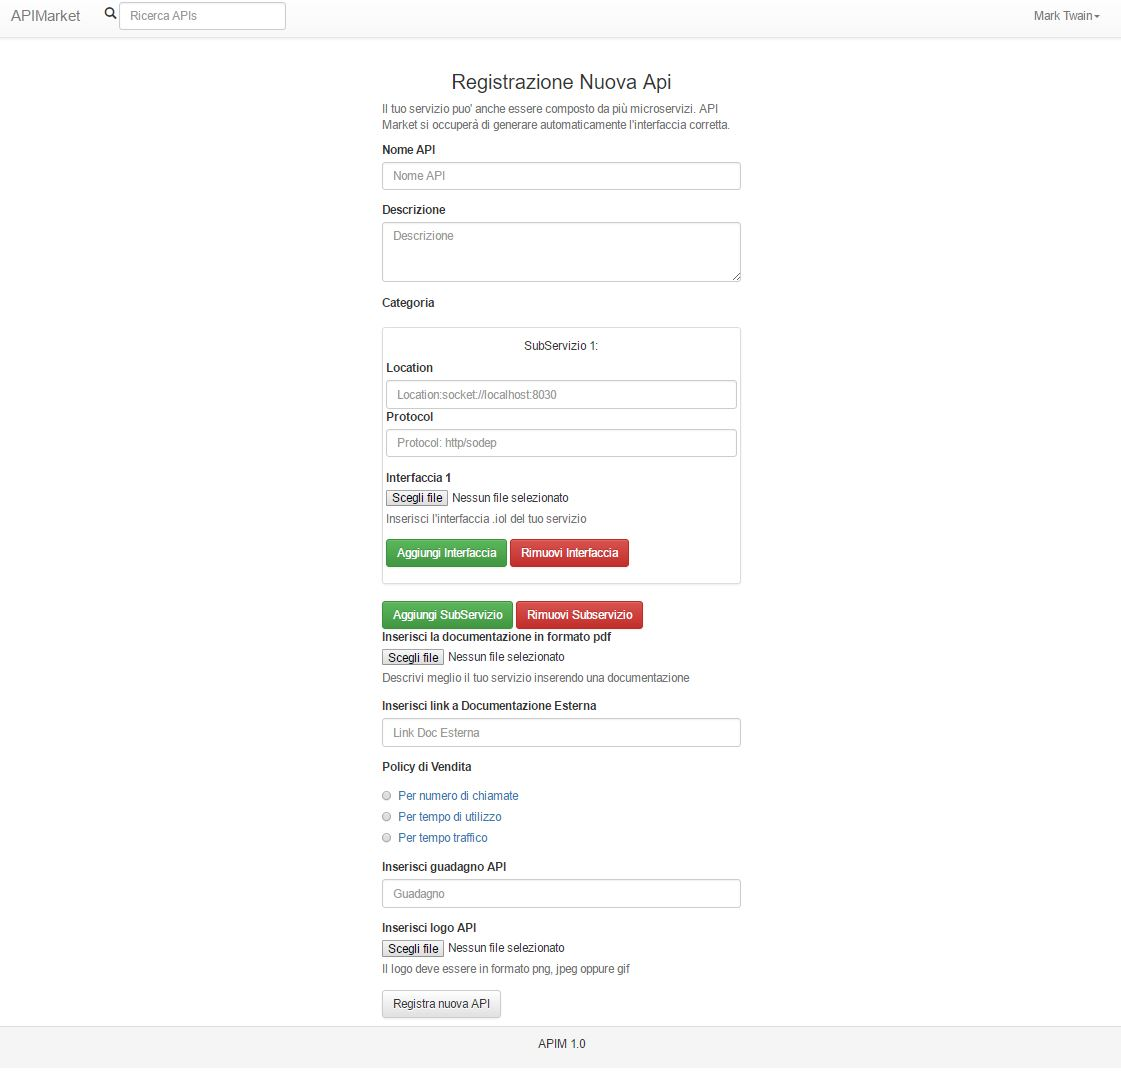
\includegraphics[scale=0.31]{img/APIM_nuovaApi.JPG}}
	\caption{Registrazione API}
\end{figure}

All'interno, l'utente dovrà specificare obbligatoriamente i seguenti dati per permettere l'inserimento del proprio prodotto nella piattaforma

\begin{itemize}
	\item Nome dell'API;
	\item Breve descrizione;
	\item Tags che identificano le categorie a cui appartiene;
	\item L'URI/Posizione del servizio;
	\item Il protocollo di comunicazione utilizzato;
	\item I file che caratterizzano l'interfaccia;
	\item Posizione, protocollo e interfaccia di eventuali sottoservizi correlati (opzionale);
	\item Documentazione PDF o link esterno;
	\item Il guadagno desiderato e la policy scelta;
	\item Il logo del prodotto.
\end{itemize}

Qualora i campi inseriti fossero corretti, il sistema segnala che la procedura è andata a buon fine.

\subsection{Pagamenti}
Lo sviluppatore accumula il guadagno della vendita delle sue API, nel suo conto personale; esso può decidere di trasferire il ricavato sul suo conto Paypal, collegato all'indirizzo email inserito nel suo profilo.
L'operazione è possibile tramite il pulsante "NOME PULSANTE" per poi completare la transazione sul sito PAYPAL???

IMMAGINE CONTO PERSONALE

%\newpage
\section{Amministratore}
	\subsection{Login admin}
	Il login admin viene effettuato su una pagina speculare al login dell'utente ma in una pagina diversa; l'utente amministratore dovrà aggiungere \url{/logi_admin} all'indirizzo del marketplate \progetto.
	\label{Login amministratore}
	\begin{figure}[H]
		\centering
		\fbox{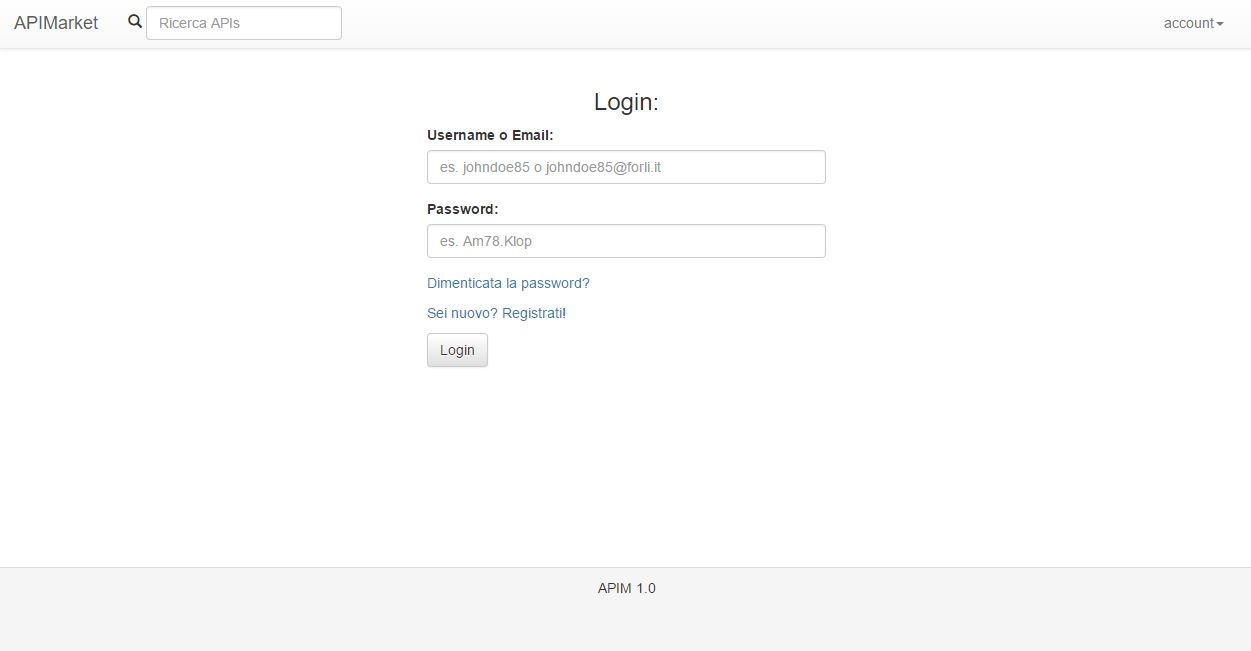
\includegraphics[scale=0.31]{img/APIM_login.JPG}}
		\caption{Login amministratore}
	\end{figure}

\subsection{Pannello amministratore}
	L'ammistratore entrerà in un pannello, dove sulla sinistra può scegliere cose moderare.
	
		\label{Pannello amministratore}
	\begin{figure}[H]
		\centering
		\fbox{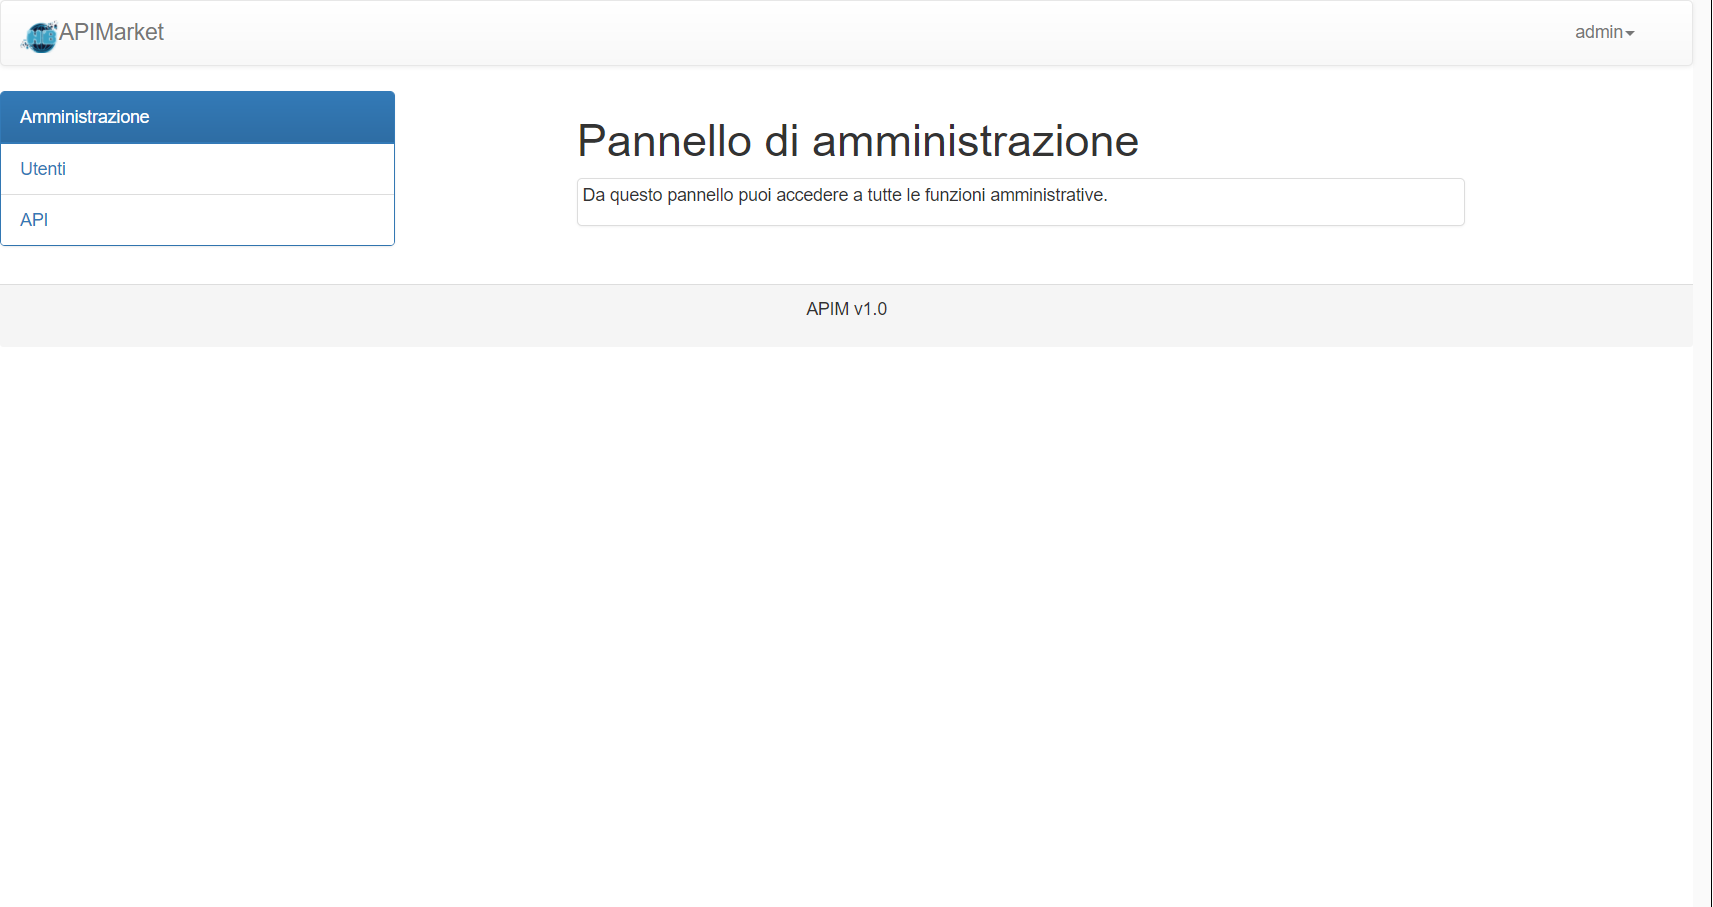
\includegraphics[scale=0.31]{img/APIM_pannelloAdmin.png}}
		\caption{Pannello amministratore}
	\end{figure}
	
	
\subsection{Moderazione API}
Selezionando la voce API, l'amministratore potrà intervenire su tutte le API presenti sul market. Le operazioni possibili sono la sospensione, attivazione e cancellazione di una API, come mostrato di seguito.

	\label{Moderazione API}
	\begin{figure}[H]
		\centering
		\fbox{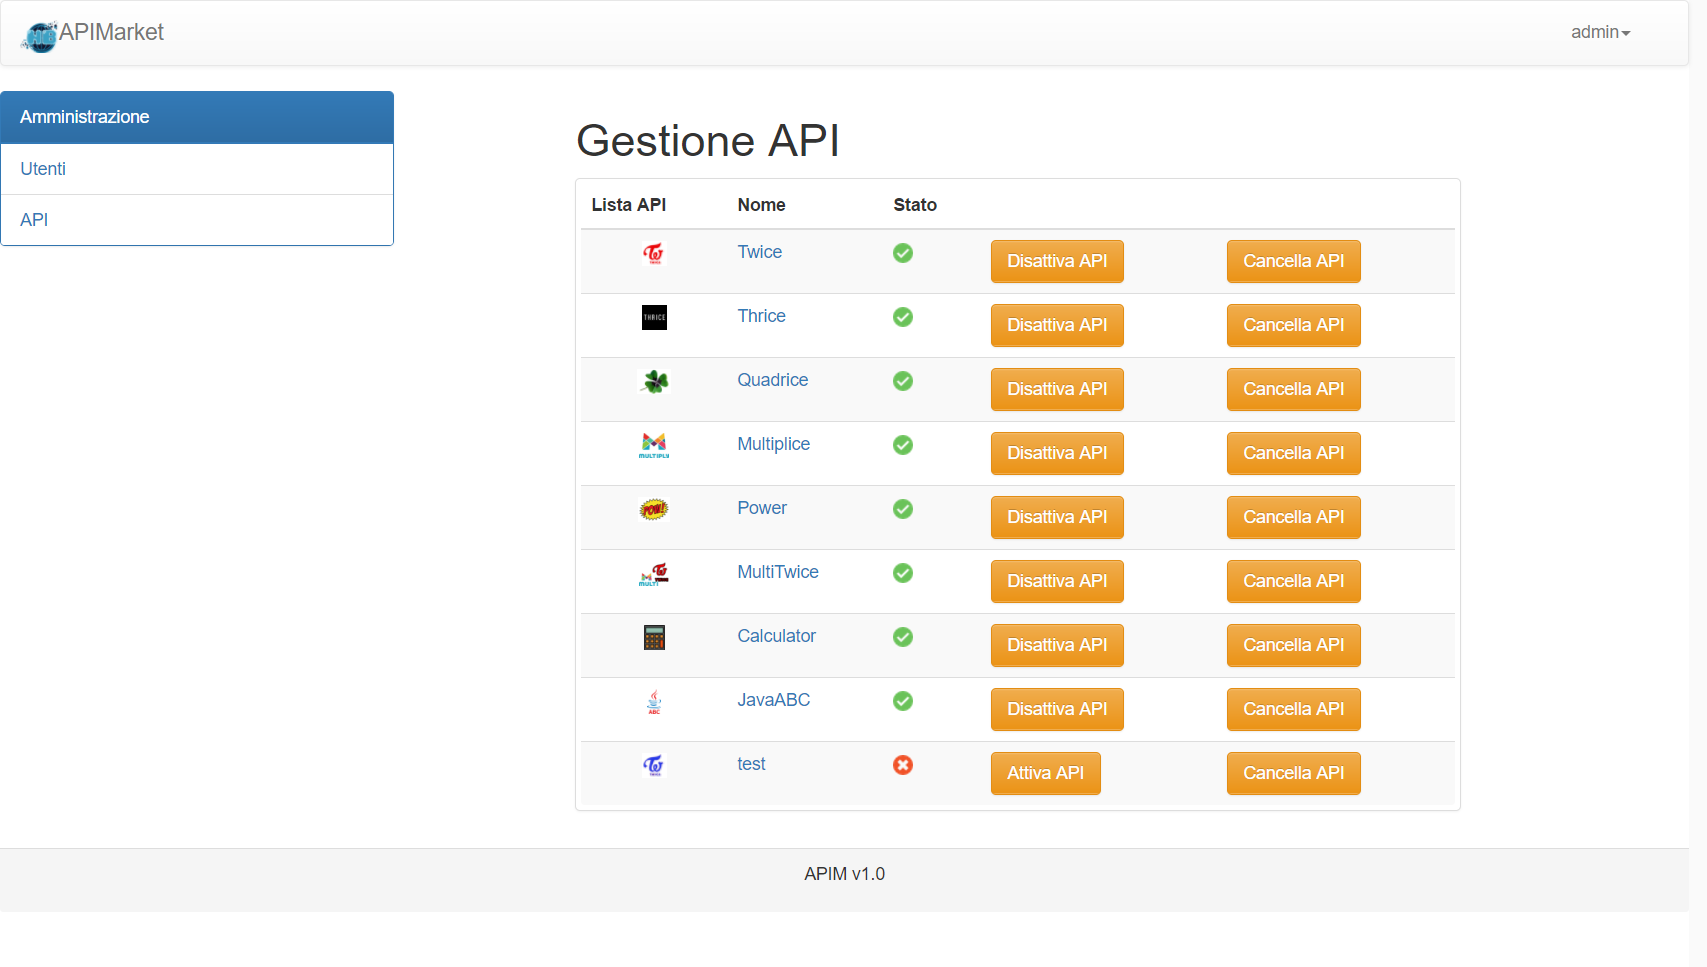
\includegraphics[scale=0.31]{img/APIM_modificaAPI.png}}
		\caption{Moderazione API}
	\end{figure}


\subsection{Moderazione Utente}
Selezionando la voce Utenti, l'amministratore potrà visualizzare le API registrate e attive di tutti gli utenti, con la possibilità di eliminare gli utenti, come mostrato nella seguente immagine.

\label{Moderazione Utente}
\begin{figure}[H]
	\centering
	\fbox{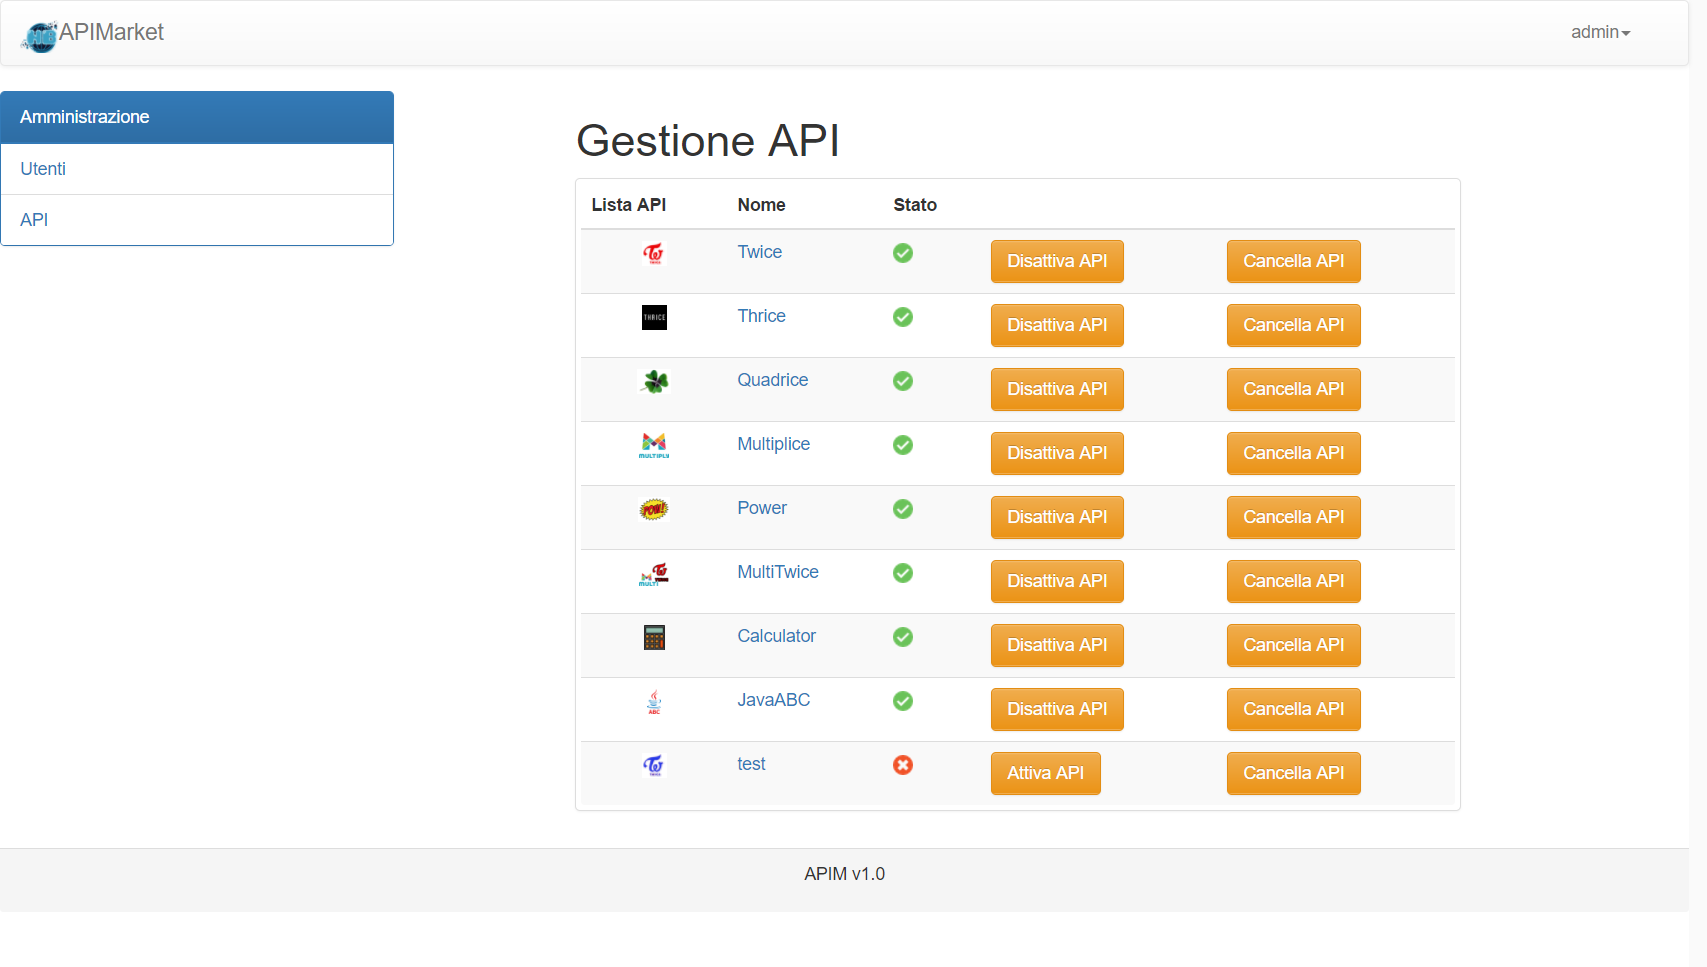
\includegraphics[scale=0.31]{img/APIM_modificaAPI.png}}
	\caption{Moderazione Utente}
\end{figure}



%%Importante: Non modificare questo template
%Modificare il documento principale per cambiare le parti

\begin{center}


%Spaziatura verticale

\vspace{4em}

%Intestazione con nome del gruppo
\begin{center} 
	\begin{Huge}
		\textbf{\fontsize{15mm}{20mm}\selectfont \gruppoLink} 
	\end{Huge}
\end{center}

\begin{center}
	\begin{Large}
		\vspace{0.3em}
		\textbf{Progetto \progetto}
	\end{Large}
\end{center}

%Inclusione del logo

\includegraphics[keepaspectratio = true,width=6cm]{../../Template/img/LogoNetbreak.png}

%Prima pagina senza intestazione né piè di pagina	
\thispagestyle{empty}

%Le informazioni del documento sono ancorate a fine pagina
\vfill

%Nome del documento
\begin{Huge} \textbf{\documento} \end{Huge}

%Tabella centrale
\begin{center}
\large\textbf{Informazioni sul documento} \\ \vspace{2em}
\small
\begin{tabular}{r l}
	\textbf{Nome del documento} & \nomedocumentofisico \\
	\textbf{Data di creazione} & \datacreazione\\
	\textbf{Ultima modifica} & \datamodifica\\
	\textbf{Versione} & \versione\\
	\textbf{Stato} & \stato \\
	\textbf{Redatto da}	& \redazione\\
	\textbf{Verificato da}	& \verifica\\
	\textbf{Approvato da}	& \approvazione\\
	\textbf{Uso}  & \uso\\
	\textbf{Distribuzione} & \gruppo \\
	\textbf{Destinato a}  &  \destinateTo \\
	\textbf{Email di riferimento}  &  \email \\
\end{tabular}
\end{center}

\vspace{2em}

\normalsize
%Inclusione abstract
\textbf{Abstract\\} 
Questo documento contiene il \PdP\ relativo al prodotto \progetto\ determinato dal gruppo \gruppo.
\end{center}
\clearpage

%\newpage
\section{Registrazione}
Per poter usufruire delle funzionalità complete dell'API Market, quali acquisto e vendita di API, è necessario registrarsi. \MakeUppercase{è} possibile registrarsi alla piattaforma premendo il pulsante preposto nella barra superiore. La schermata che apparirà all'utente sarà la seguente:

\label{Registrazione}
\begin{figure}[H]
	\centering
	\fbox{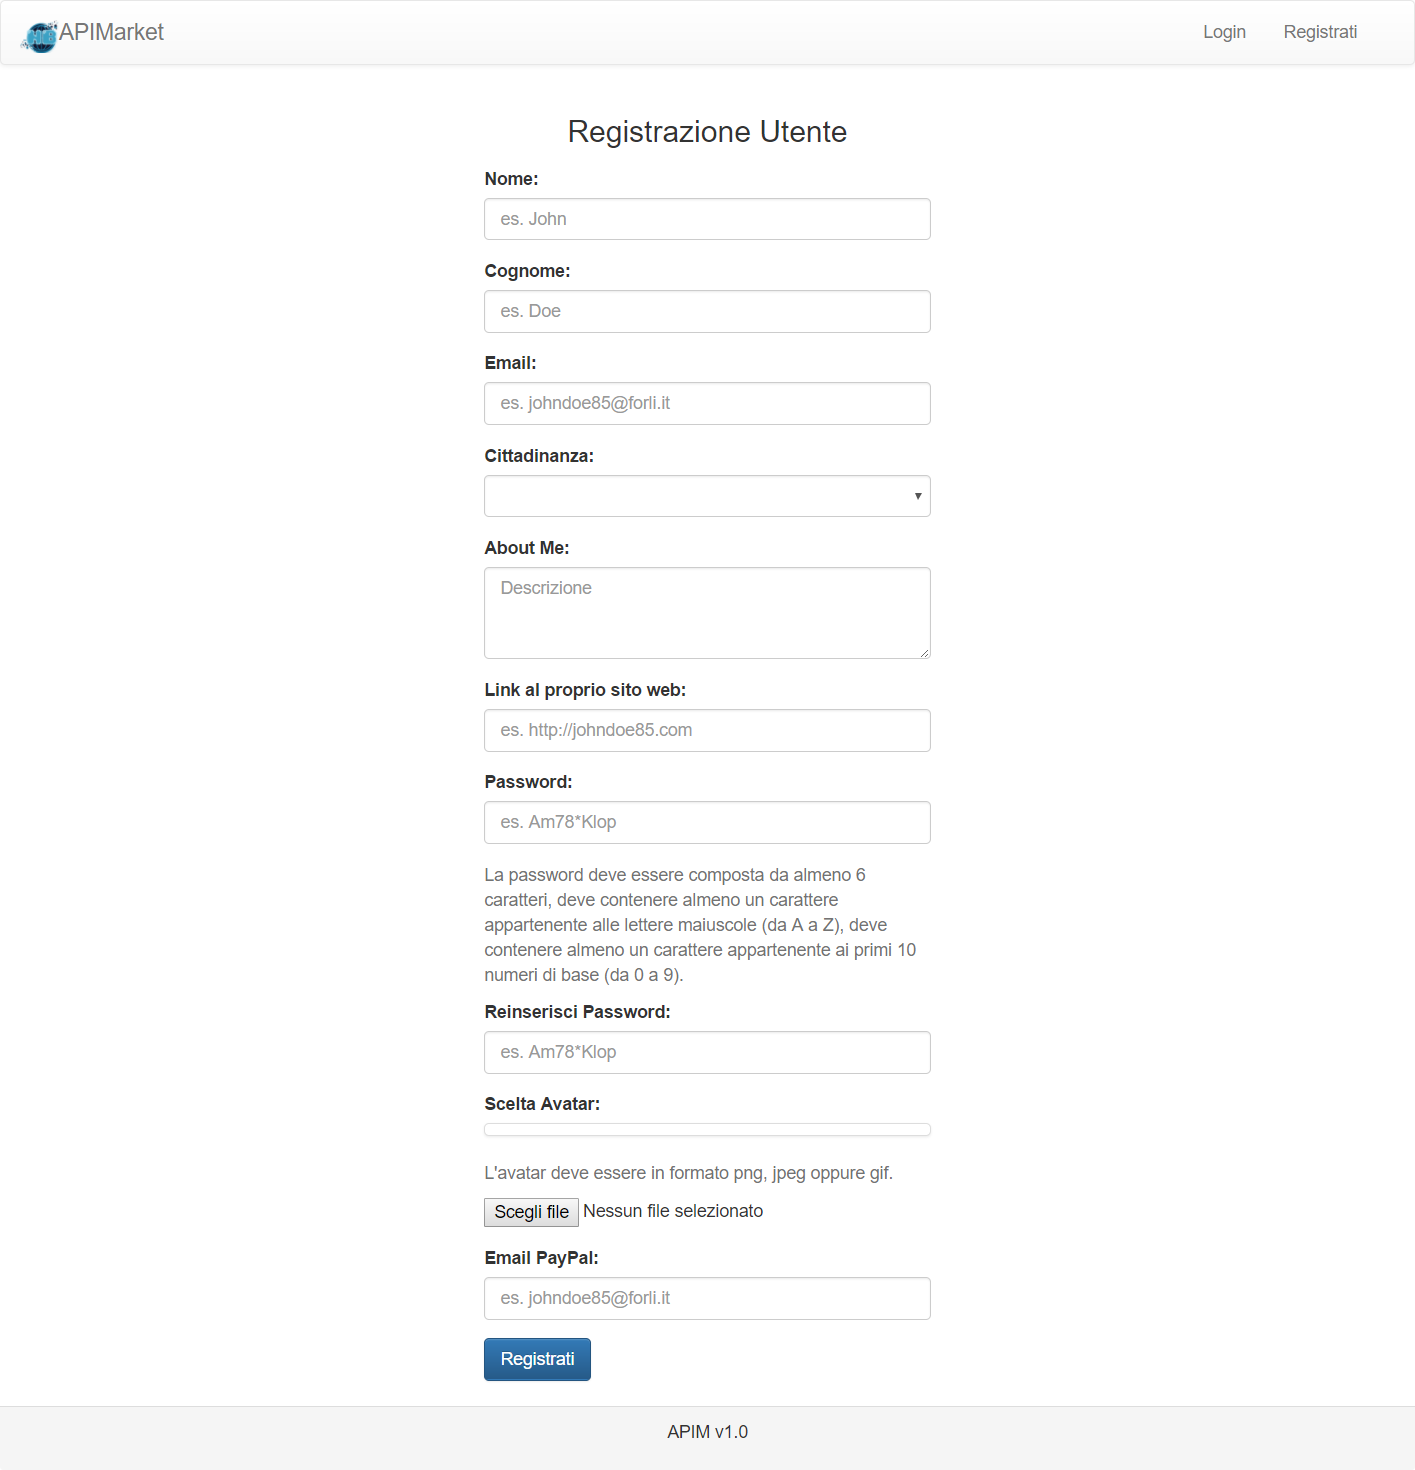
\includegraphics[scale=0.31]{img/APIM_registrazione.JPG}}
	\caption{Registrazione}
\end{figure}

un utente per registrasi dovrà compilare correttamente i seguenti campi, che sono obbligatori:
\begin{itemize}
	\item Nome;
	\item Cognome;
	\item Username desiderato;
	\item Stato di residenza;
	\item Indirizzo e-mail;
	\item Password desiderata;
	\item Conferma password.
\end{itemize}

Qualora questi dati non fossero presenti o corretti, il sistema segnala un errore all'atto di registrazione e l'utente deve inserire dei parametri validi nei campi indicati. Sono presenti inoltre dei campi opzionali:

\begin{itemize}
	\item Descrizione personale;
	\item Immagine personale;
	\item Email PayPal.
\end{itemize}

Questi campi, seppur non obbligatori, bloccano la registrazione qualora il loro inserimento non fosse effettuato in modo corretto. Si prega di prestare attenzione ai requisiti visualizzati nella schermata di registrazione.

\subsection{Login}

Tramite la barra superiore, vicino al pulsante di registrazione è possibile effettuare il login. La schermata di login può essere visualizzata a partire da ogni pagina non autenticata, selezionando l'apposita voce.
Il login può essere effettuato da un utente precedentemente registrato e dalla schermata di login è possibile autenticarsi nella piattaforma per poter svolgere le funzionalità preposte agli utenti registrati. 

\label{Login}
\begin{figure}[H]
	\centering
	\fbox{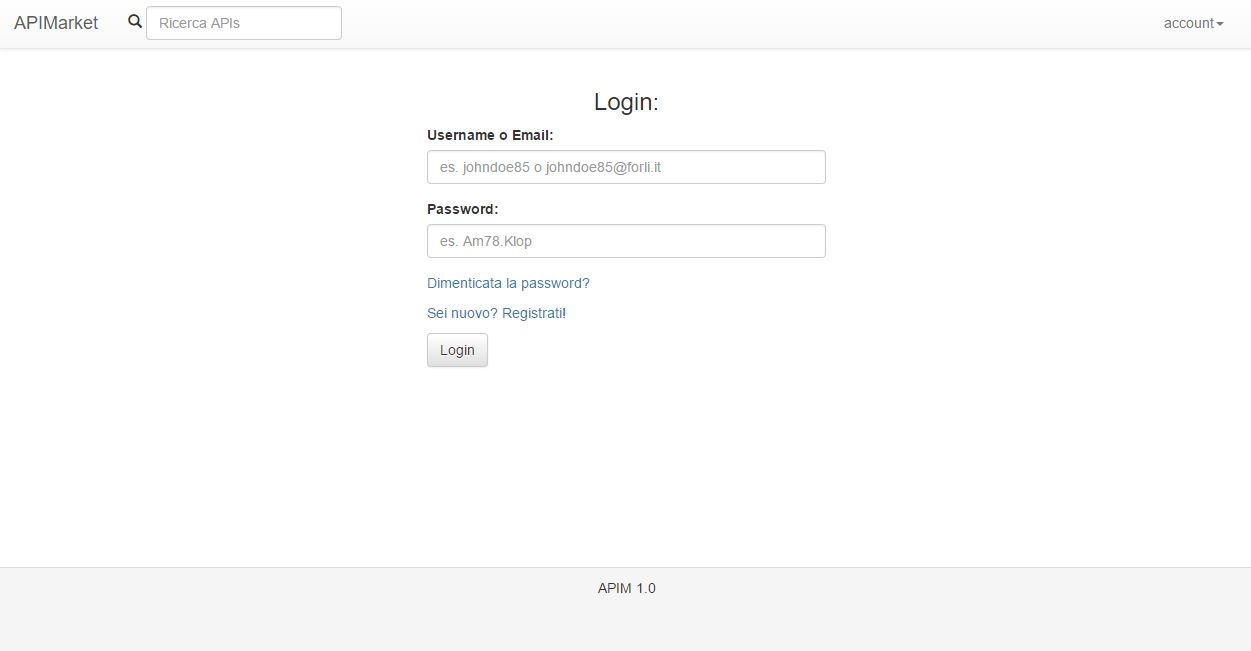
\includegraphics[scale=0.31]{img/APIM_login.JPG}}
	\caption{Login}
\end{figure}

\subsection{Conferma Login}
Dopo aver inserito i dati di login e cliccato sul pulsante "Login", se i dati di accesso sono corretti, l'utente visualizza una pagina di conferma login, con la possibilità di recarsi sulla Homepage oppure nella gestione del proprio profilo.

\label{Conferma Login}
\begin{figure}[H]
	\centering
	\fbox{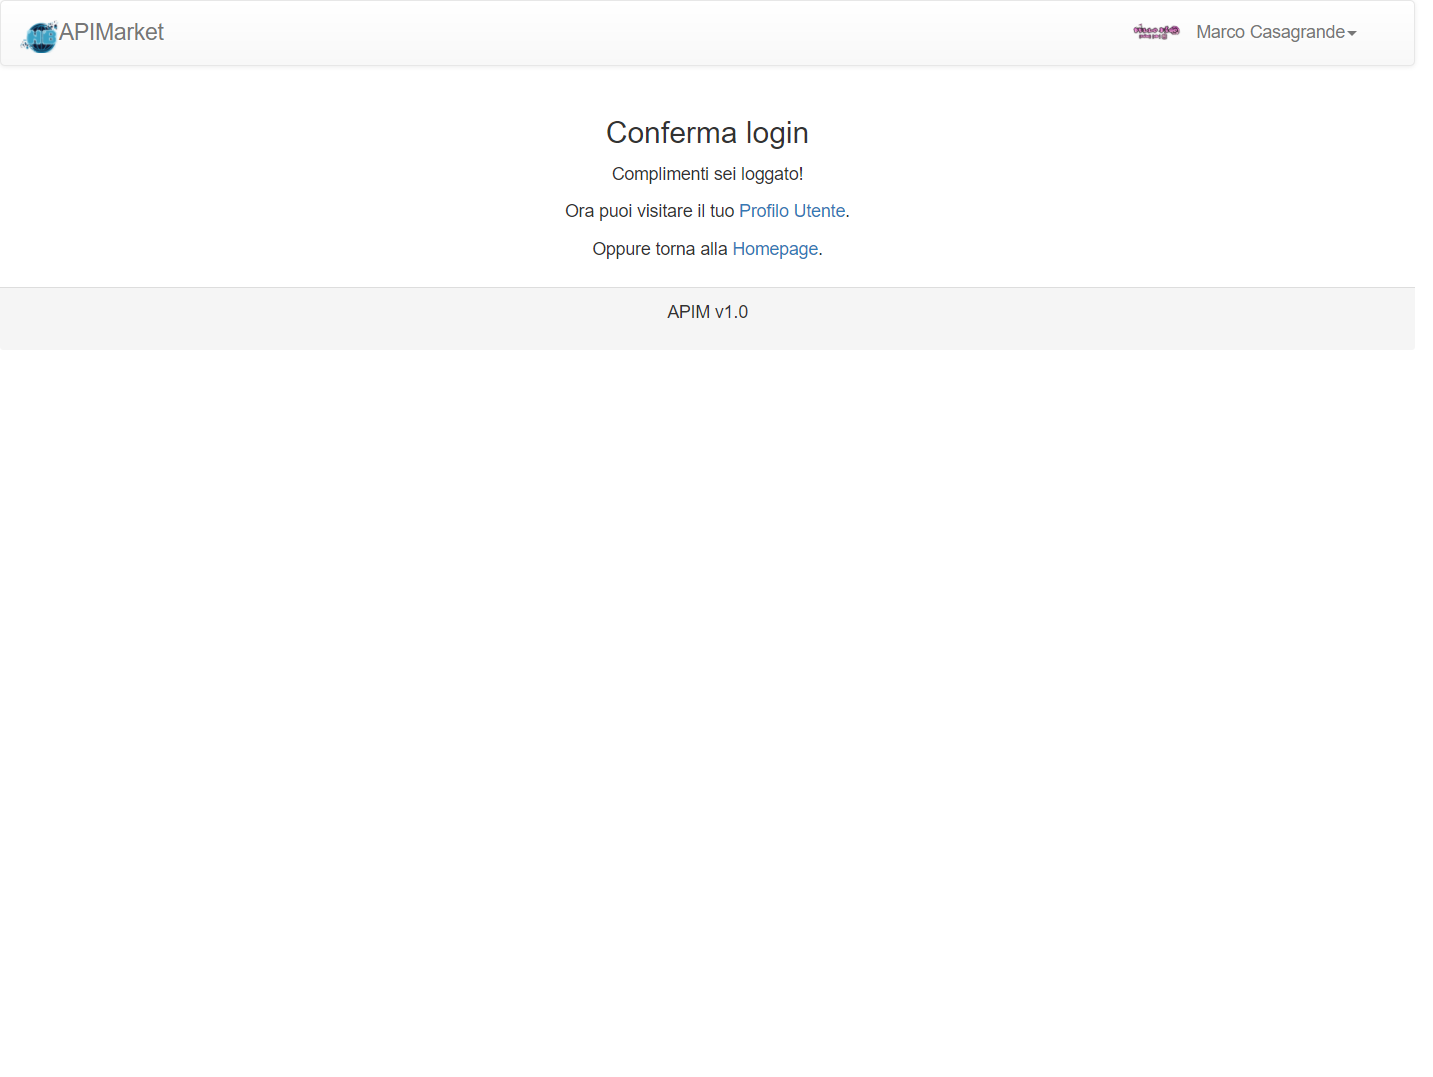
\includegraphics[scale=0.31]{img/APIM_confermaLogin.jpg}}
	\caption{Login}
\end{figure}



\subsection{Recupero Password}
Qualora si fosse dimenticata la password, dalla schermata di login si può accedere alla pagina per il recupero della password. Inserendo l'indirizzo email si può ottenere un link per reimpostare i propri dati personali tramite una pagina dedicata. 

\label{Recupero Password}
\begin{figure}[H]
	\centering
	\fbox{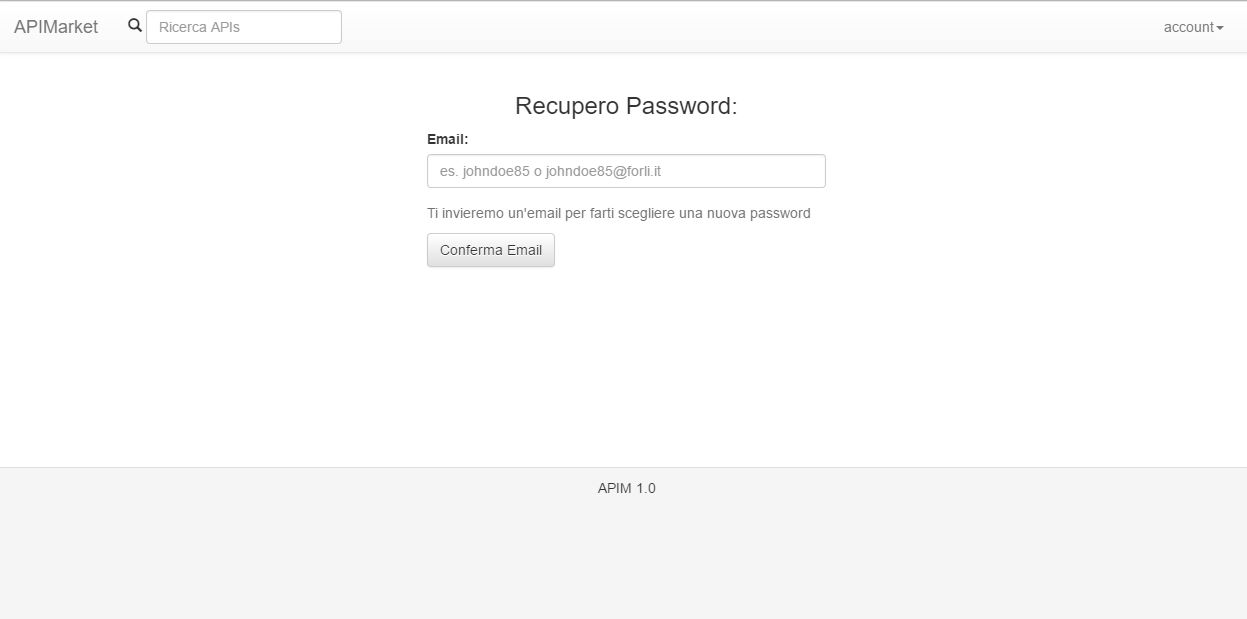
\includegraphics[scale=0.31]{img/APIM_recuperoPSW.JPG}}
	\caption{Recupero Password}
\end{figure}

%\newpage
\section{Profilo utente}

\subsection{Gestione profilo}

Una volta effettuato il login, è possibile accedere al proprio profilo utente. La schermata principale relativa al profilo apparirà come nella figura sottostante.

\label{Profilo utente}
\begin{figure}[H]
	\centering
	\fbox{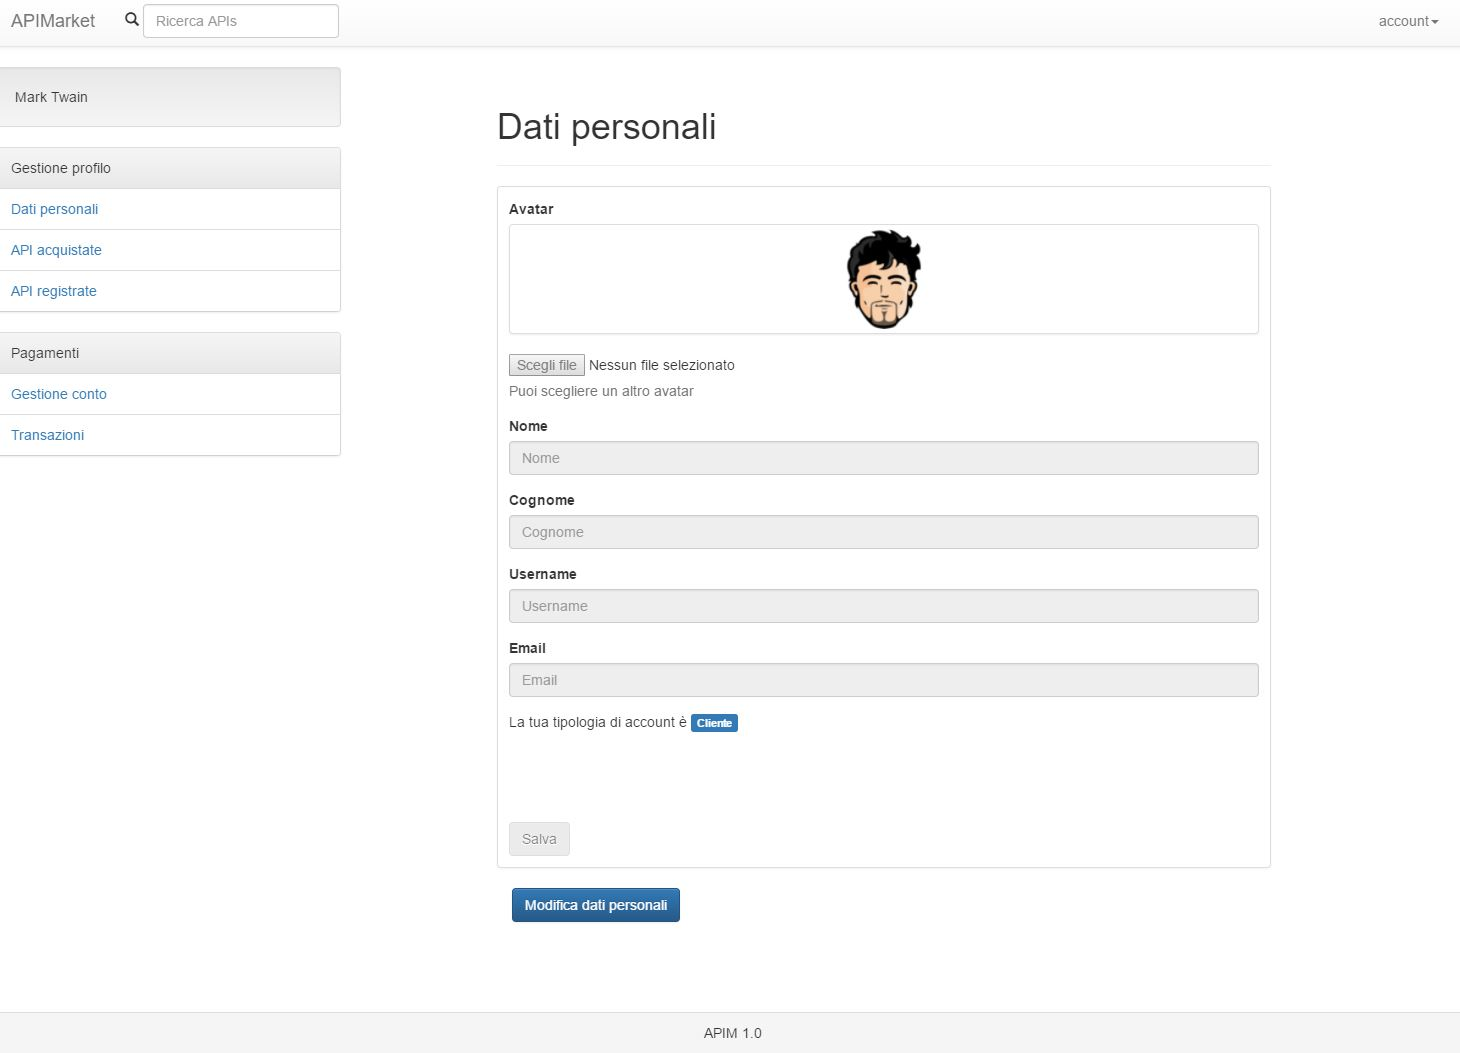
\includegraphics[scale=0.52]{img/APIM_account.JPG}}
	\caption{Profilo utente}
\end{figure}

Dalla schermata si potranno modificare i dati personali, inseriti al momento della registrazione, quali la propria anagrafica o dati relativi all'account quali l'immagine personale. E' visualizzato inoltre a quale gruppo di utenza si appartiene: l'utente registrato semplice infatti è un utente denominato "cliente", mentre l'utente abilitato al caricamento e alla vendita di servizi è denominato utente "sviluppatore".

Tramite il menù laterale è possibile navigare nelle schermate del proprio profilo. Clickando sulla voce API acquistate si potrà consultare l'elenco delle api attualmente in possesso o acquistate in passato con i relativi dati. 

\label{API acquistate}
\begin{figure}[H]
	\centering
	\fbox{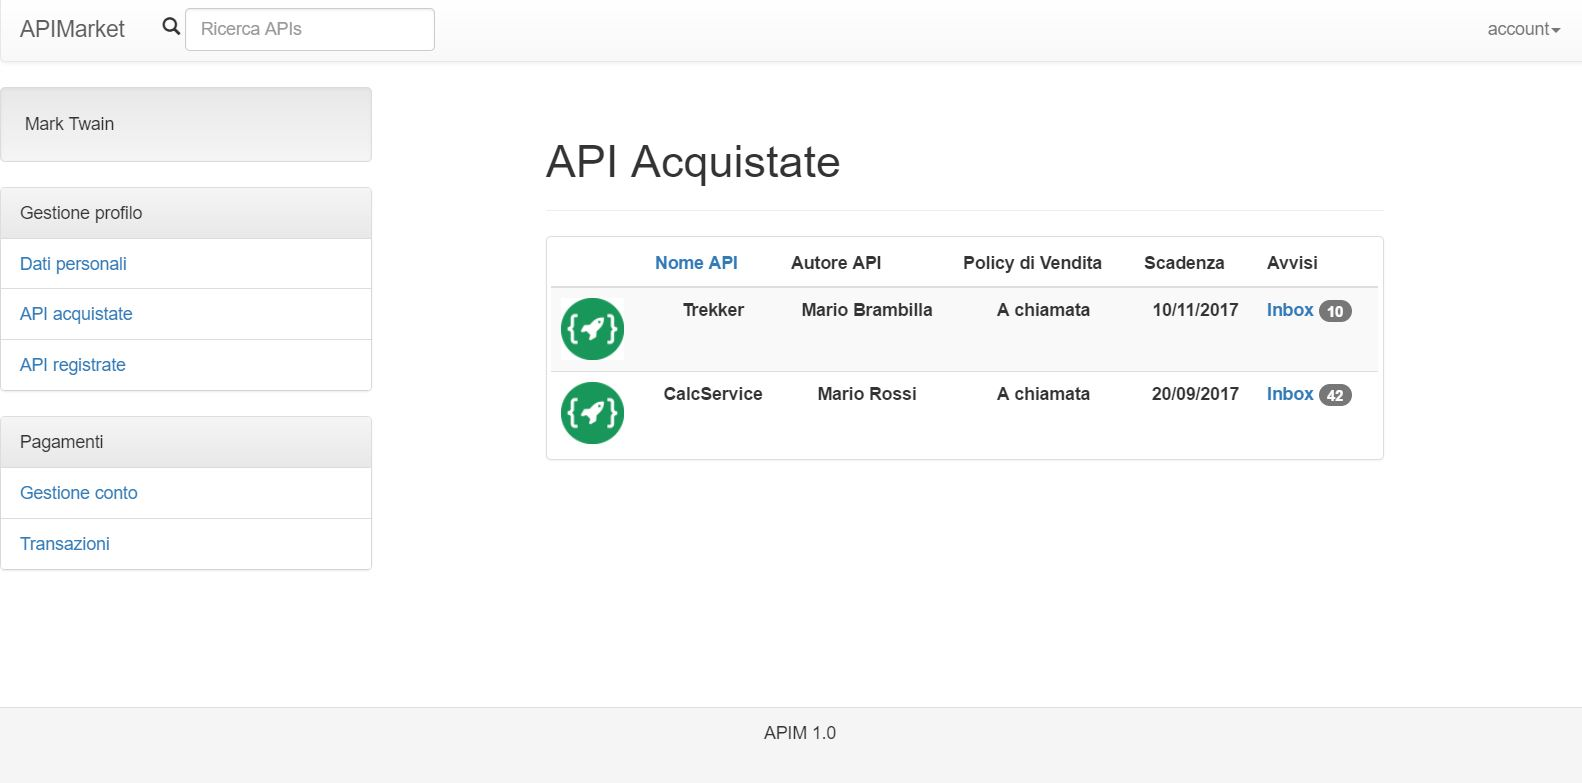
\includegraphics[scale=0.47]{img/APIM_apiAcquistate.JPG}}
	\caption{API acquistate}
\end{figure}

Qualora l'utente appartenga alla categoria "sviluppatore", è disponibile la voce relativa alle API registrate con relative statistiche.

\label{API registrate}
\begin{figure}[H]
	\centering
	\fbox{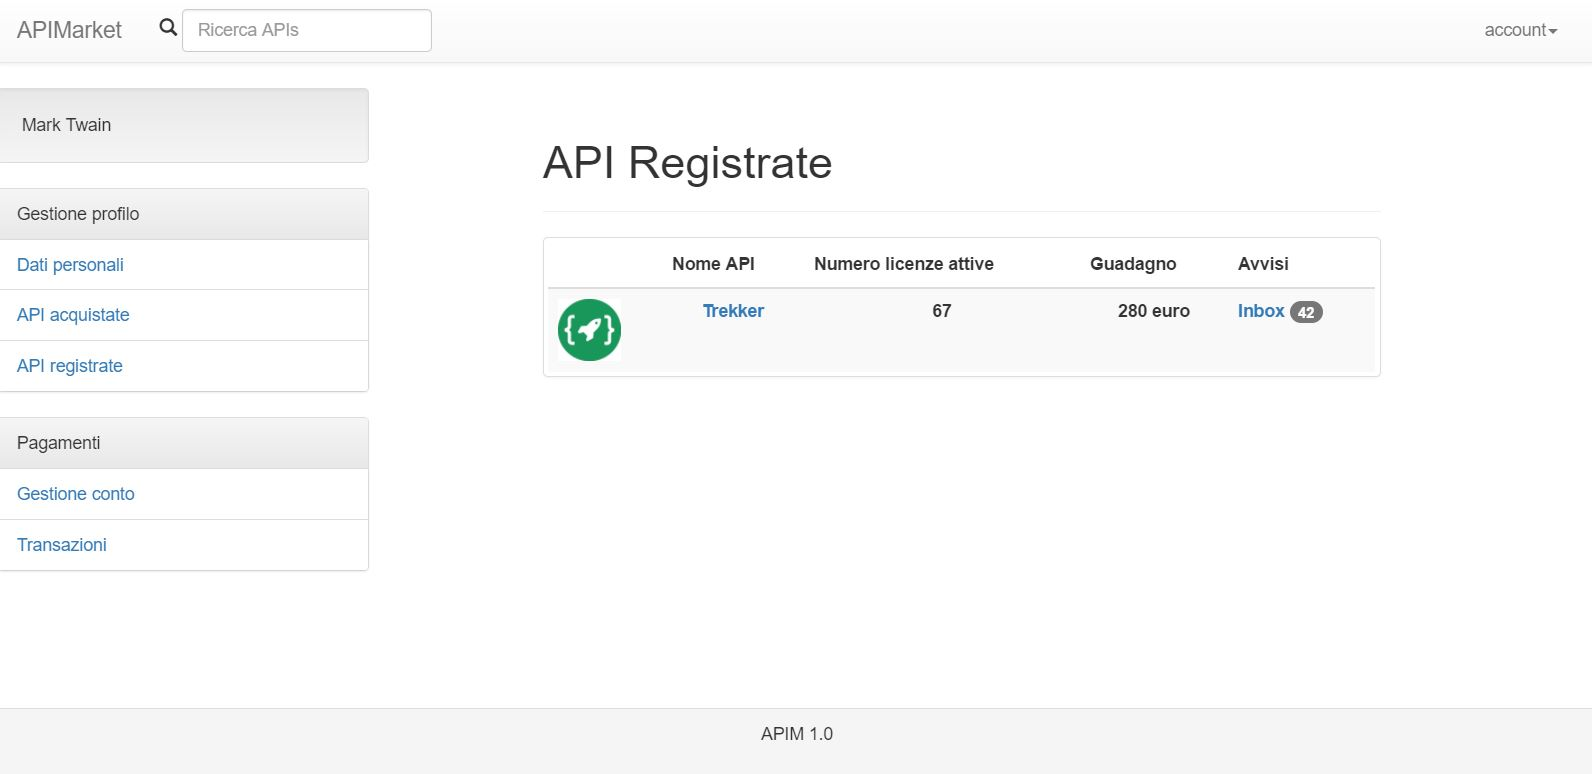
\includegraphics[scale=0.47]{img/APIM_apiRegistrate.JPG}}
	\caption{API registrate}
\end{figure}

\subsection{Registrazione API}

L'utente abilitato alla vendita (Sviluppatore) può  registrare le proprie API per la vendita nell'apposita pagina accessibile dal profilo utente. La schermata per la registrazione di nuove API appare come mostrato nell'immagine sottostante.

\label{Registrazione API}
\begin{figure}[H]
	\centering
	\fbox{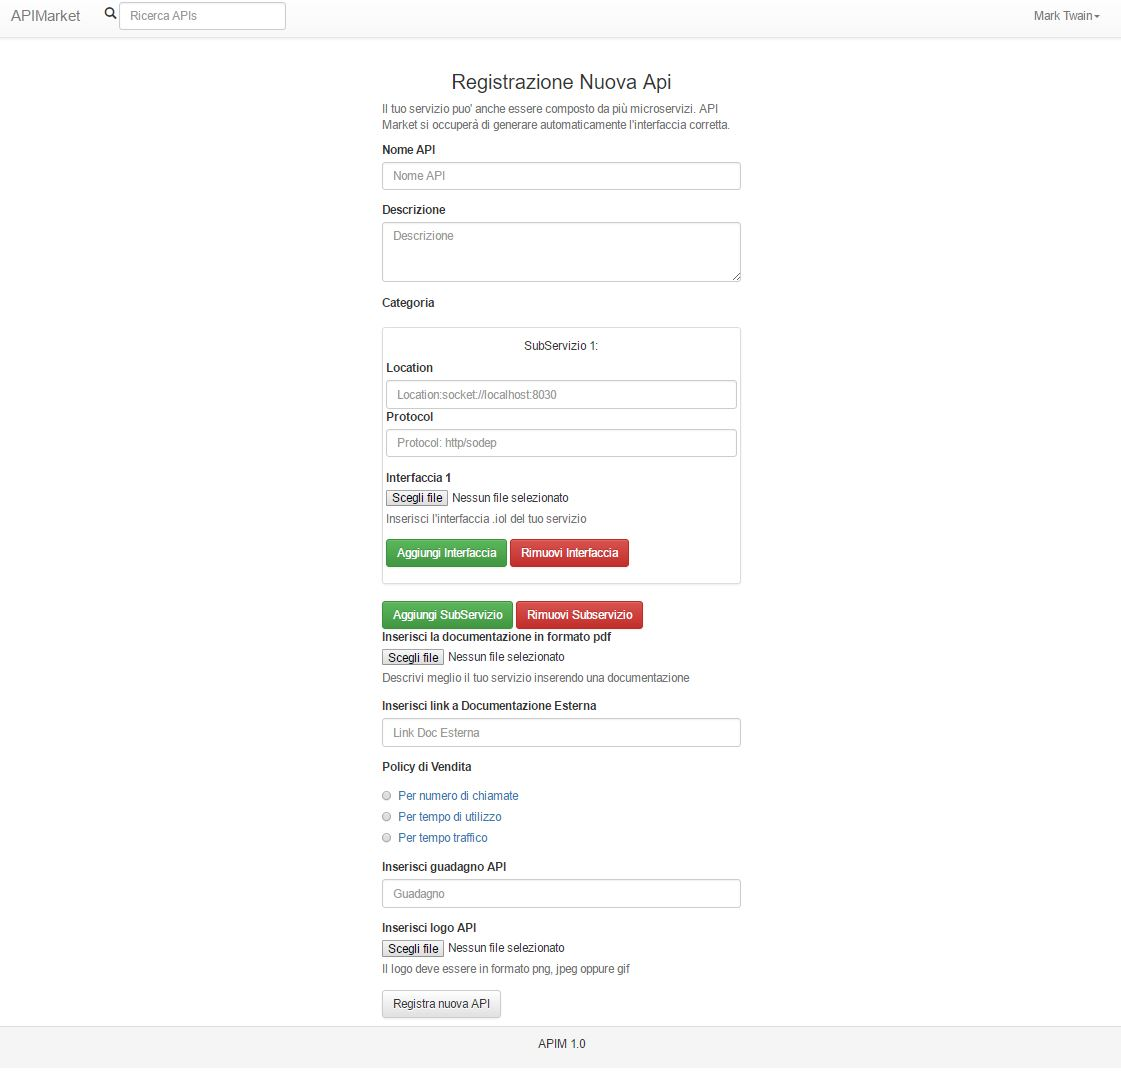
\includegraphics[scale=0.65]{img/APIM_nuovaApi.JPG}}
	\caption{Registrazione API}
\end{figure}

All'interno, l'utente dovrà specificare obbligatoriamente i seguenti dati per permettere l'inserimento del proprio prodotto nella piattaforma

\begin{itemize}
	\item Nome dell'API;
	\item Breve descrizione;
	\item Tags che identificano le categorie a cui appartiene;
	\item L'URI/Posizione del servizio;
	\item Il protocollo di comunicazione utilizzato;
	\item I file che caratterizzano l'interfaccia;
	\item Posizione, protocollo e interfaccia di eventuali sottoservizi correlati (opzionale);
	\item Documentazione PDF o link esterno;
	\item Il guadagno desiderato e la policy scelta;
	\item Il logo del prodotto.
\end{itemize}

Qualora i campi inseriti fossero corretti, il sistema segnala che la procedura è andata a buon fine.

\subsection{Pagamenti}

Gli utenti sviluppatori possono consultare i propri dati finanziari, quali movimenti o saldo, nelle sezioni preposte del proprio profilo. La sezione Gestione conto mostra il saldo attuale e offre la possibilità di caricare il proprio saldo tramite funzionalità esterne (PayPal).

\label{Gestione conto}
\begin{figure}[H]
	\centering
	\fbox{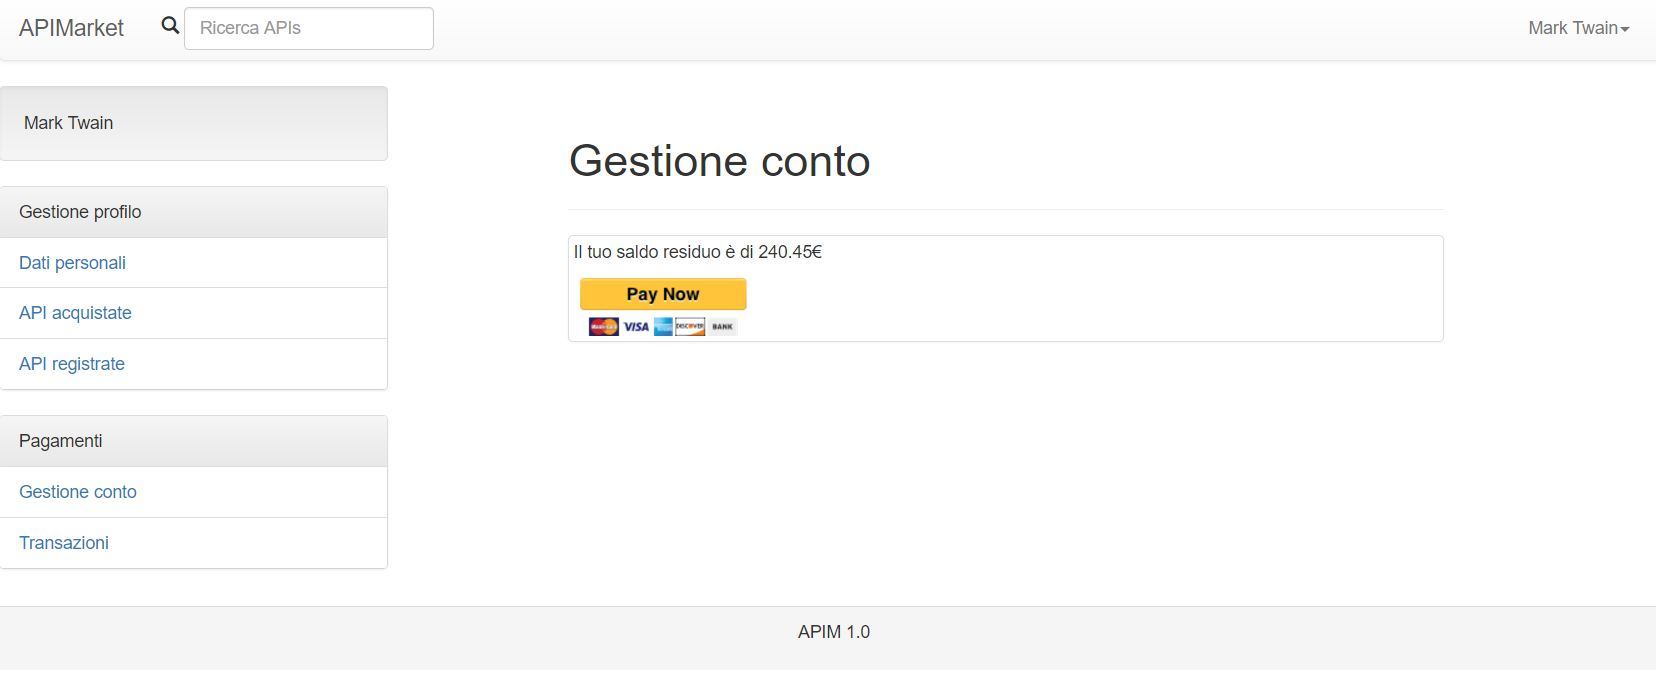
\includegraphics[scale=0.45]{img/APIM_gestioneConto.JPG}}
	\caption{Gestione conto}
\end{figure}

Nella voce transazioni, invece, è disponibile uno storico delle transazioni effettuate nell'API Market. Esse riguardano i servizi utilizzati e le relative chiamate, o gli addebiti per policy di altra tipologia. Lo storico contiene la designazione dell'API che è stata utilizzata, il costo, e la data. Esiste inoltre un ID univoco della transazione, per poter referenziare una particolare transazione con lo staff API Market.

\label{Transazioni}
\begin{figure}[H]
	\centering
	\fbox{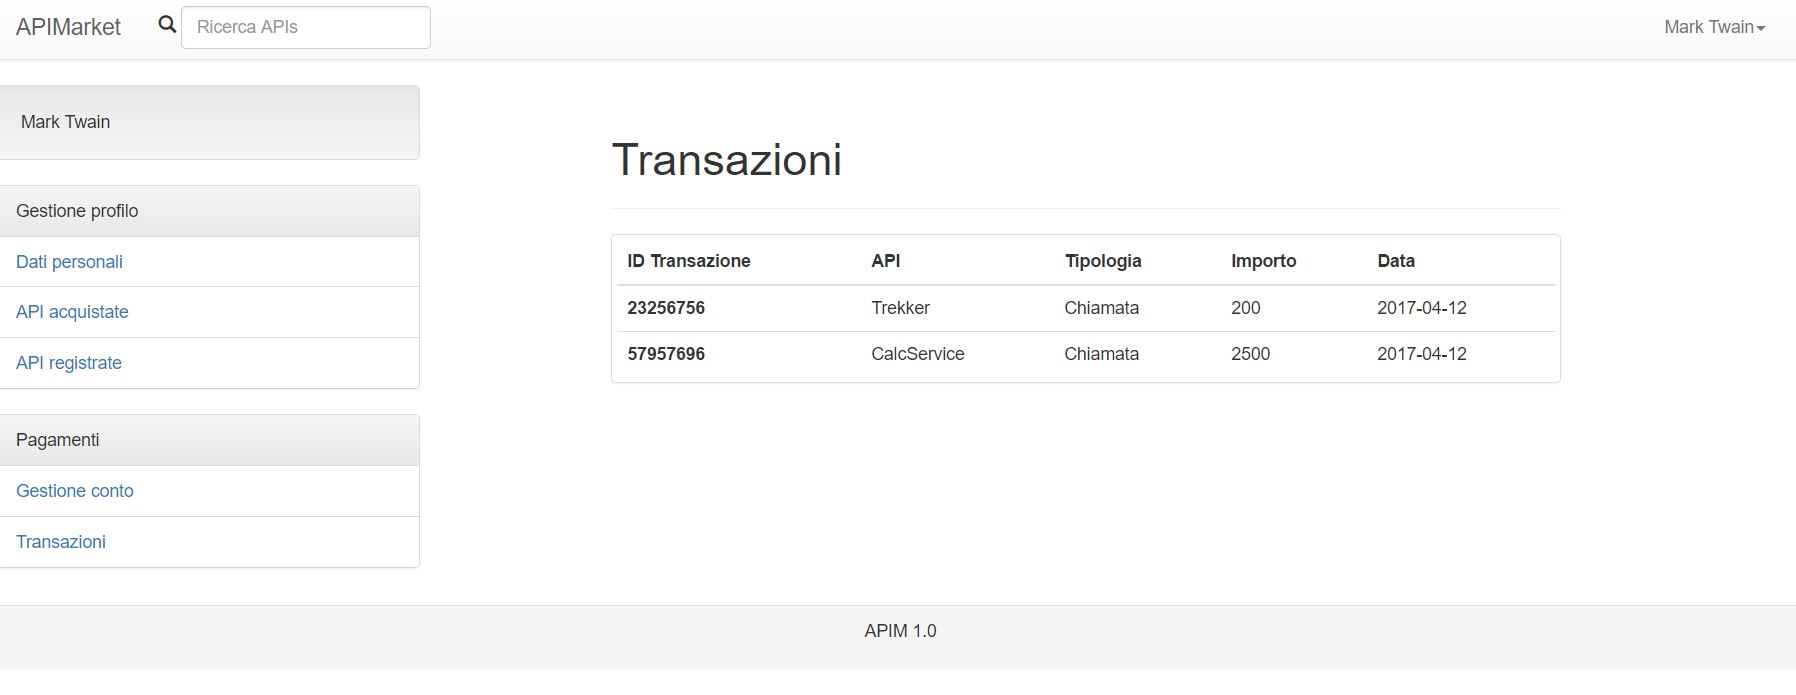
\includegraphics[scale=0.42]{img/APIM_transazioni.JPG}}
	\caption{Transazioni}
\end{figure}
%\newpage

%\newpage
\section{Ricerca e visualizzazione API}

\subsection{Ricerca}
La funzionalità di ricerca è disponibile per qualsiasi categoria di utente. Essa permette, in base ad una parola chiave, di visualizzare le API relative contenute nella piattaforma. In seguito a ricerca, effettuata scrivendo sull'apposita barra la parola chiave desiderata, si può accedere ad un elenco dei risultati come mostrato.

\label{Risultati ricerca}
\begin{figure}[H]
	\centering
	\fbox{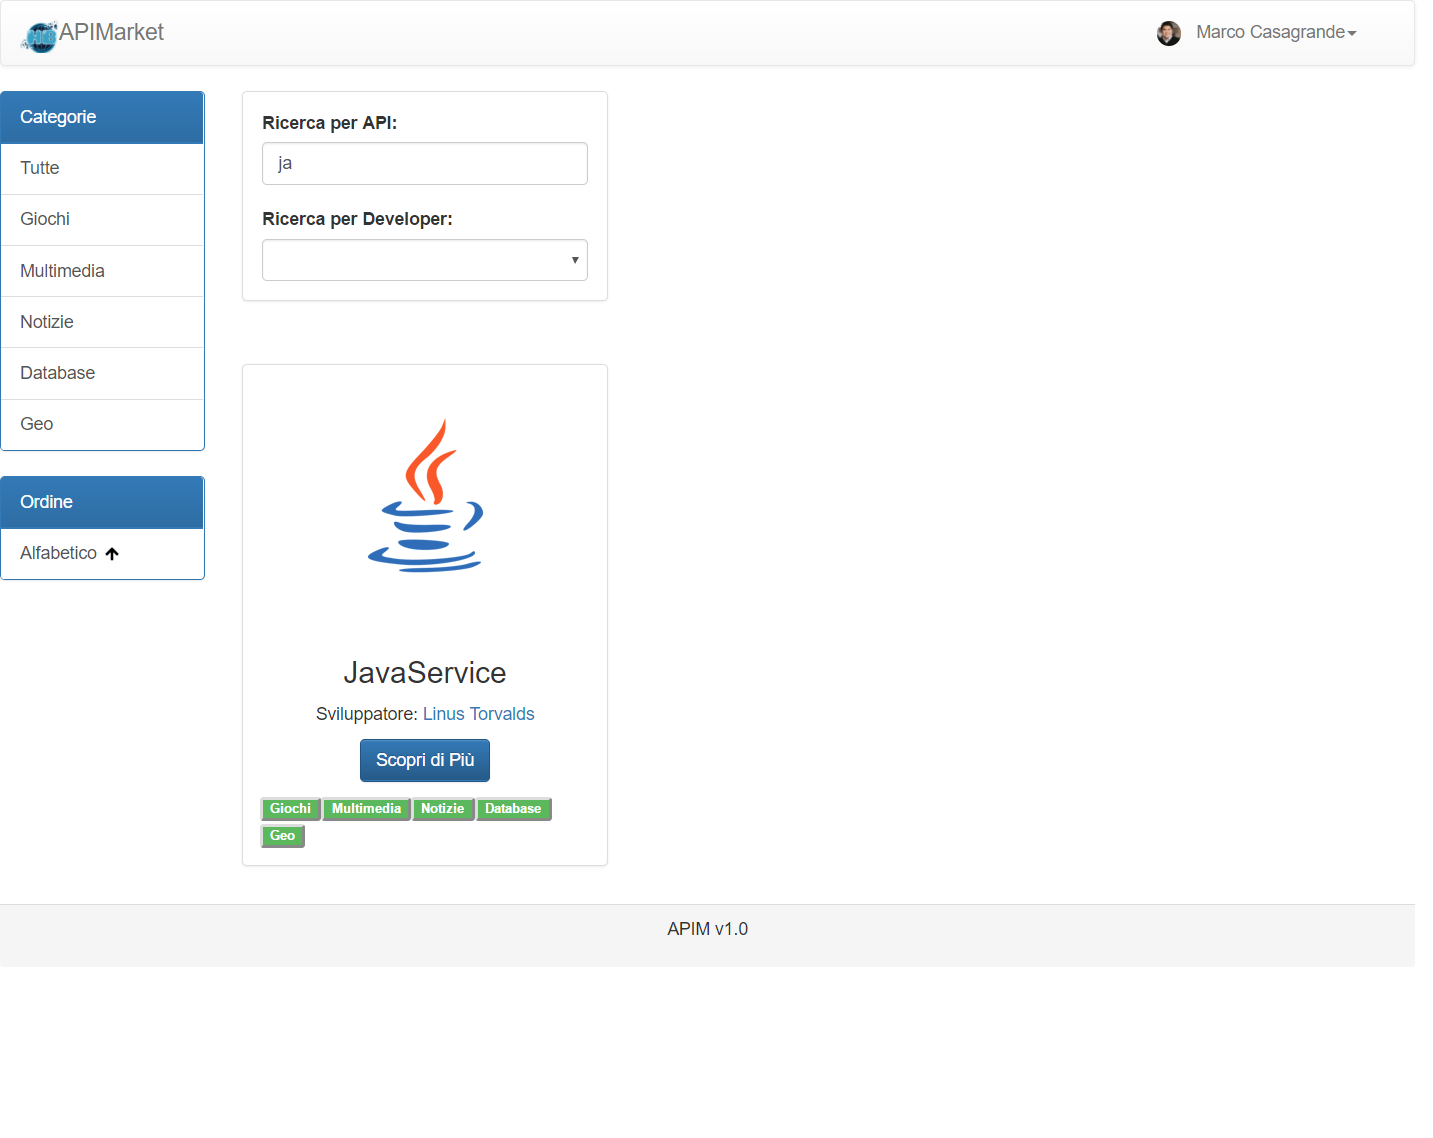
\includegraphics[scale=0.31]{img/APIM_ricerca.JPG}}
	\caption{Risultati ricerca}
\end{figure}

Selezionando un API dall'elenco dei risultati, è possibile visualizzare i dati nel dettaglio, con relative specifiche. 

\label{Visualizzazione API}
\begin{figure}[H]
	\centering
	\fbox{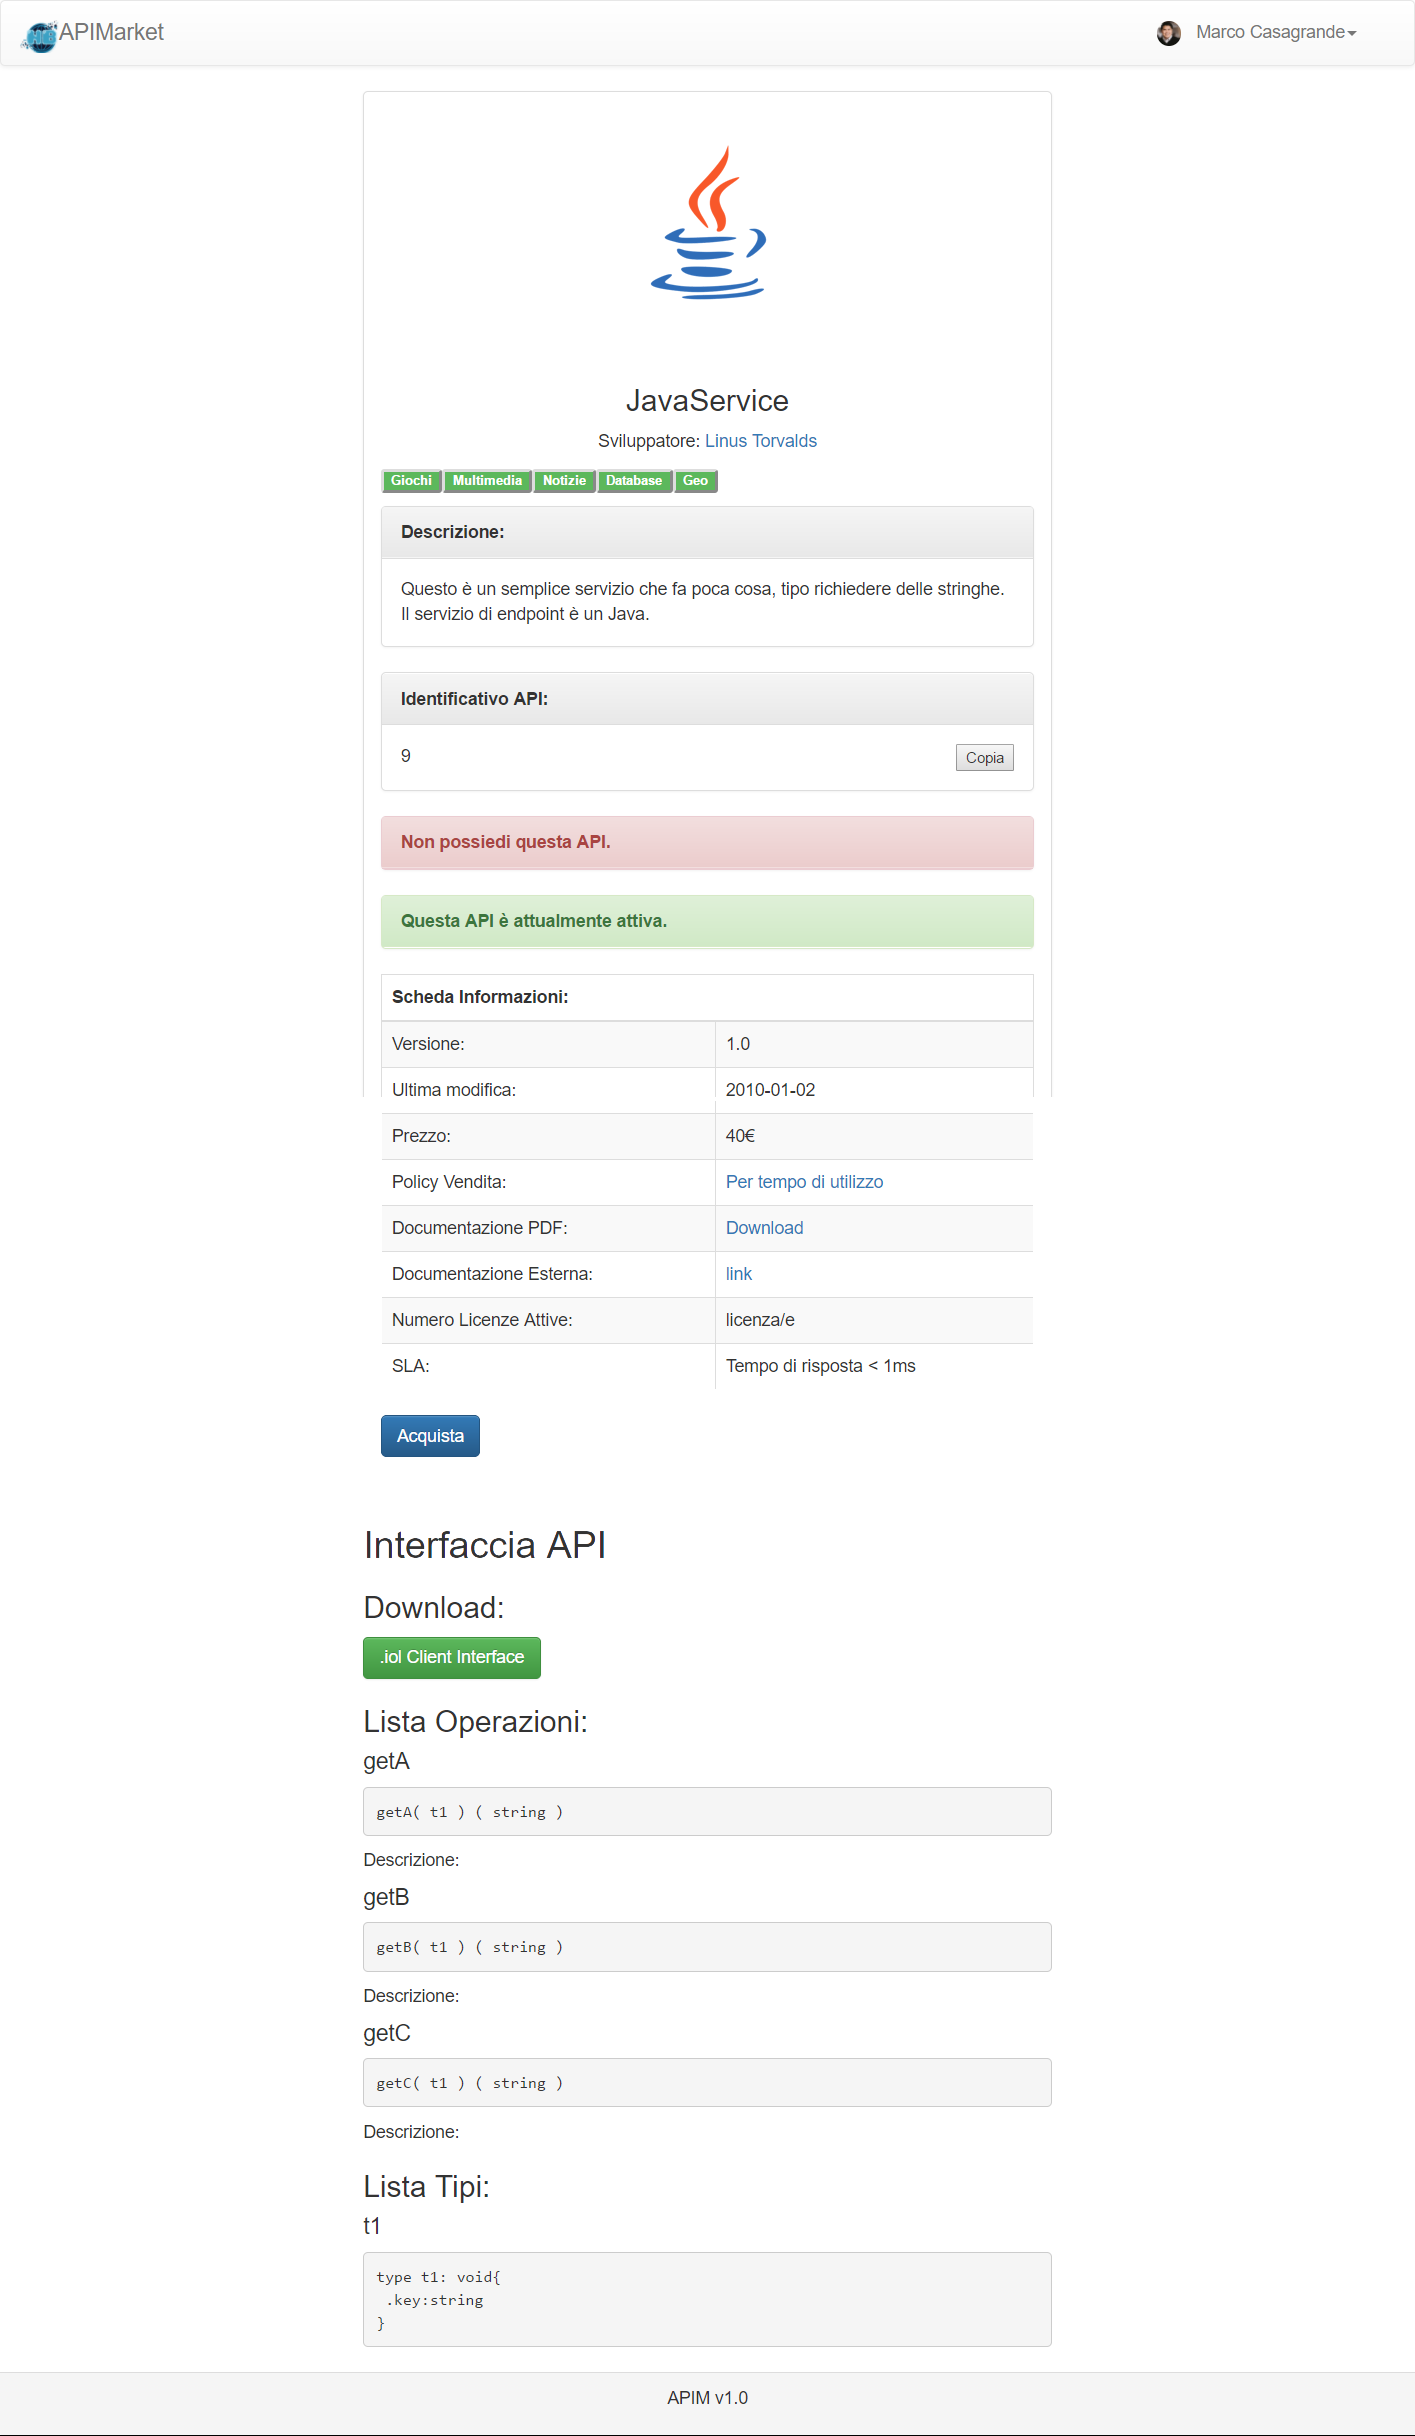
\includegraphics[scale=0.28]{img/APIM_dettagliApi.png}}
	\caption{Visualizzazione API}
\end{figure}

Ciascuna API presente nella piattaforma è caratterizzata da una policy di vendita, descritta all'interno di ciascun prodotto. E' possibile visualizzare i dettagli della policy clickando sull'apposito link nella schermata.

\label{Visualizza policy API}
\begin{figure}[H]
	\centering
	\fbox{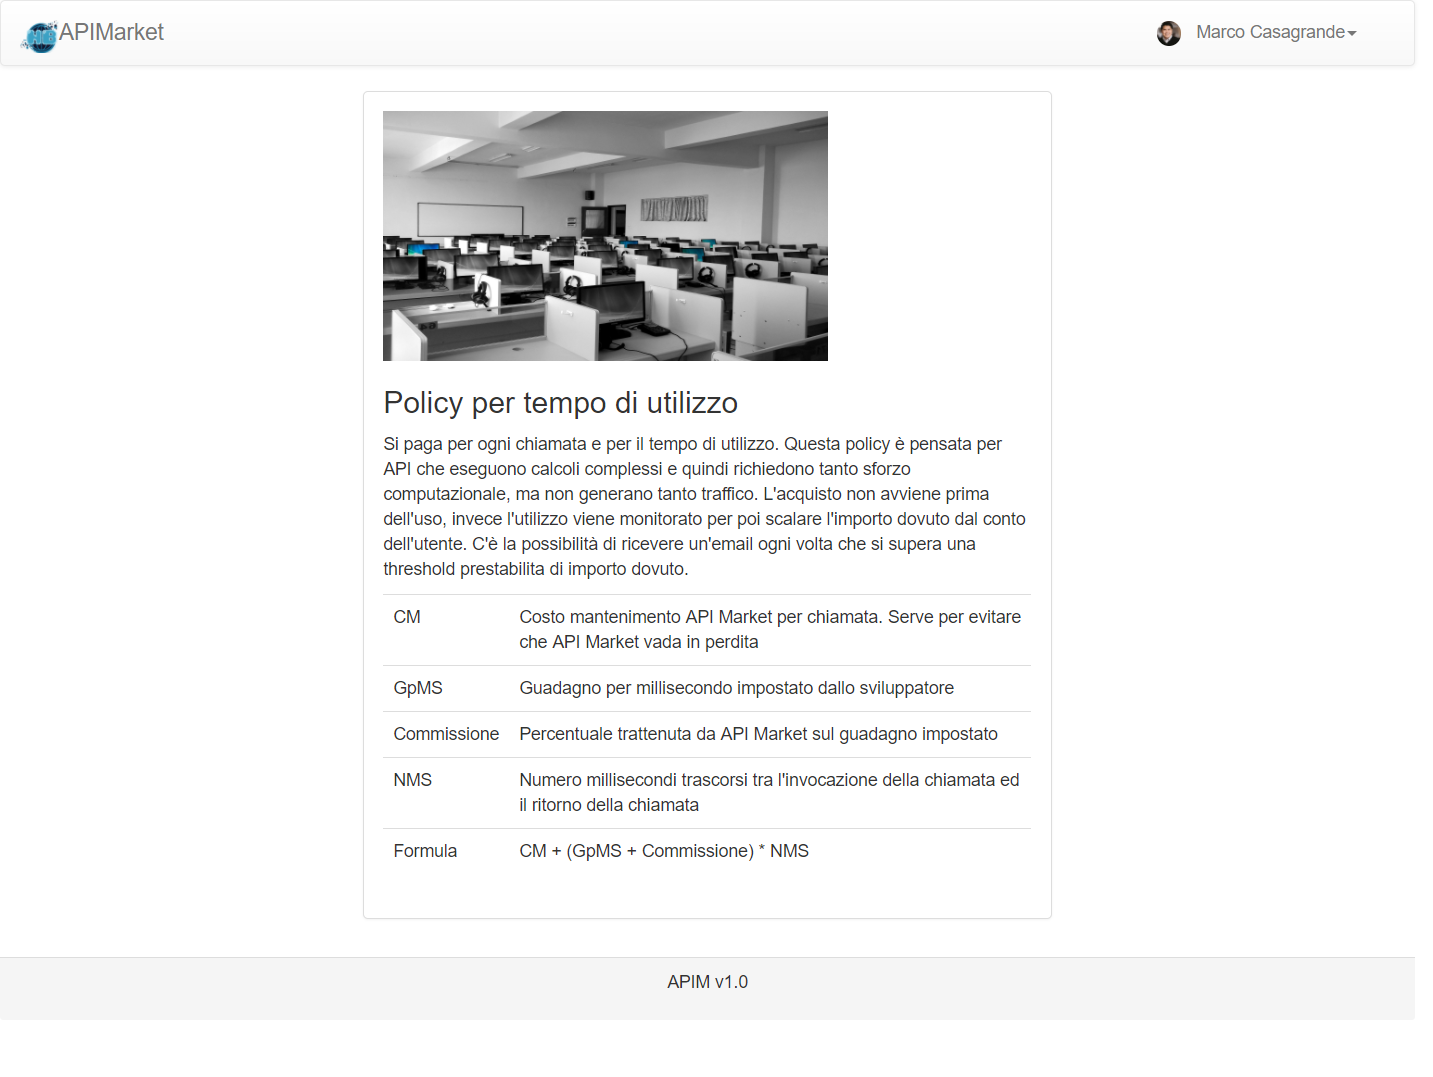
\includegraphics[scale=0.31]{img/APIM_policy.JPG}}
	\caption{Visualizza policy API}
\end{figure}

Qualora si decidesse di effettuare l'acquisto, nella schermata è presente un pulsante Acquista che porterà alla schermata relativa al completamento della transazione se l'utente è loggato, altrimenti chiederà di effettuare il login o la registrazione. L'utente riceverà un API key con la quale potrà utilizzare il servizio acquistato. Nella pagina relativa al completamento della transizione, l'utente potrà scegliere l'importo da acquistare a seconda della policy dell'API che intende acquistare. 

\label{Acquisto API}
\begin{figure}[H]
	\centering
	\fbox{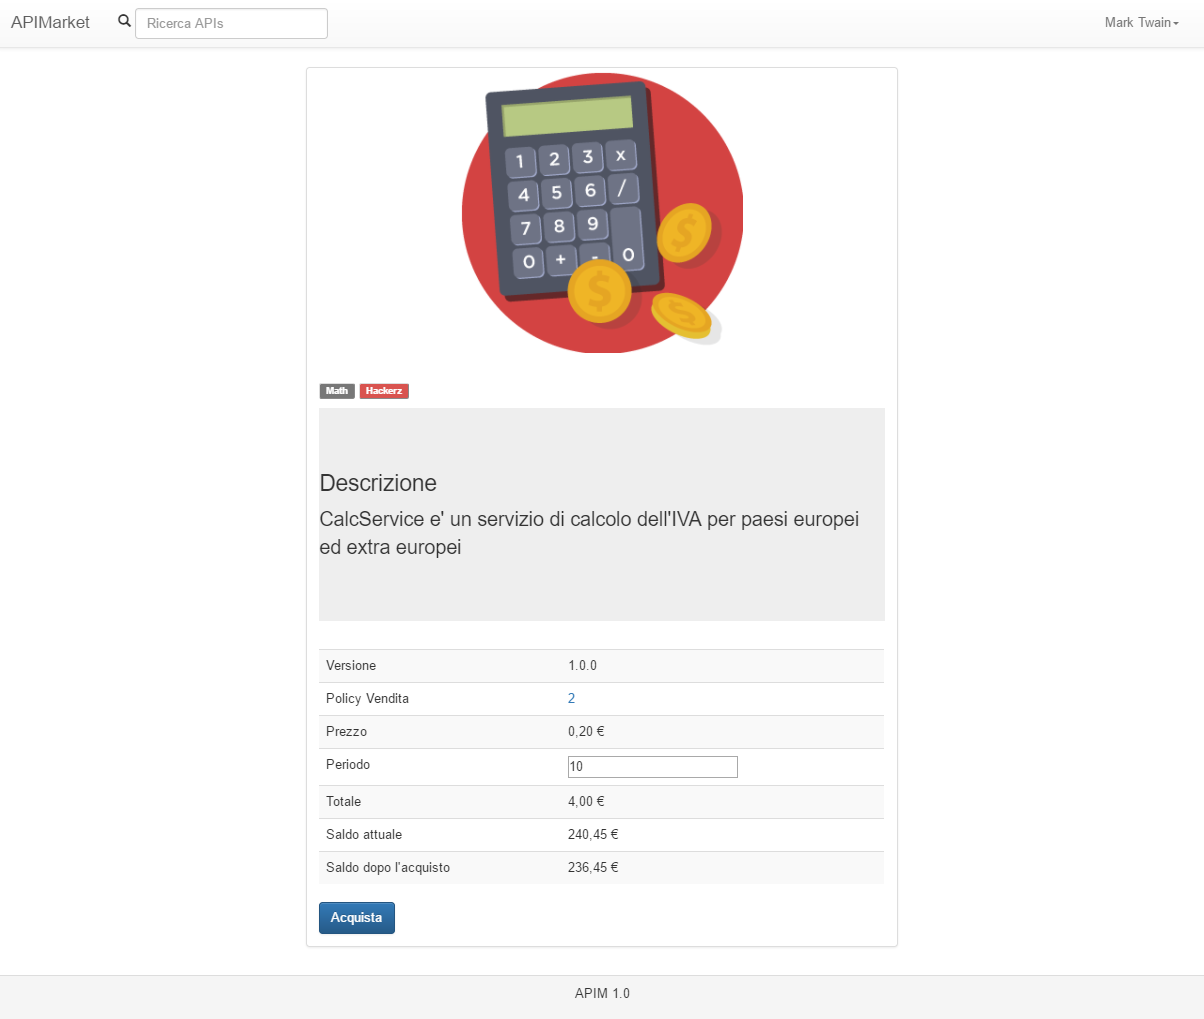
\includegraphics[scale=0.60]{img/APIM_acquisto.PNG}}
	\caption{Acquisto API}
\end{figure}



\end{document}